\chapter{Constructing landscape-level $R_0$-maps}
\label{ch:6-adb}

Previously in chapter \ref{ch5:dispersal-model}, we considered a generic $SIR$-based non-local dispersal model (NLM) that spread via a Gaussian dispersal. 
The NLM resolved the major problem witnessed in section \ref{fig:ch4_uk_spread}, 
namely, the failure of the percolation-based model to spread on a realistic host density. 
However, Chapter \ref{ch5:dispersal-model} and the NLM lacked biological specificity.
The present chapter aims to construct a simplified $SEIR$ model of ash dieback capturing only the essential dynamics of wind-borne dispersal.
Ash dieback (ADB), caused by the fungus \textit{Hymenoscyphus fraxineus}, poses a threat to the survival of European ash (\textit{F. excelsior})\textemdash
the reader is referred to section \ref{ch2:ash-dieback} for a more in-depth discussion of ADB symptoms, life-cycle and management.

In section \ref{sec:seir-model}, a seasonal-based $SEIR$-like model is developed to simulate the natural wind-dispersal mechanism of ash dieback at local-spatial scales. 
The $SEIR$ model is then examined in section \ref{sec:seir-behaviour}, before outlining an effective reproduction number in section \ref{sec:SEIR-R0-definition}.
Then, in section \ref{sec:r0-map-construct} a framework is developed to spatially-scale up the local-scale model over Great Britain (GB) using a modelled ash canopy cover data-set \cite{hill.data}.
The framework is mainly generic, and could in principle, be adapted for any dispersal-based tree pathosystem\textemdash provided that a sufficient host abundance data-set is available.
Combining two models at different spatial scales has clear analogies to a sub-grid model \cite{sub-grid}.
 
A spatially explicit reproductive ratio, denoted by $R_0$, is computed from model simulations to measure invasiveness.
Critically, the wind-dispersal model of ADB relies on $R_0$  measured over an appropriate spatio-temporal scale.
The value of $R_0$ is projected onto the map of ash canopy cover data-set given by \cite{hill.data}.
From an $R_0$-map, a simplified notion of epidemic impact can be visualised through an '$R_0$-cluster' over the ash population.

The local-scale epidemic model demonstrates that long-distance dispersal (LDD) and long-term survival (i.e. persistence)  
can occur even below the threshold $R_0=1$.
Additionally, model analysis at the landscape-level reveals the size of susceptible $R_0$-clusters grow most rapidly over a narrow range of infectivity parameters.
The result of this chapter presents how the epidemic scale can vary significantly with slight deviations of epidemic parameters, 
thus supporting the call for a risk-based approach to modelling the spread of epidemics in tree populations.

\section{A spatially-explicit seasonal $SEIR$ model}
\label{sec:seir-model}

In this chapter, only the `teleomorphic' sexual reproduction of \textit{H. fraxineus} is reflected in the $SEIR$ model.
Sexual reproduction of ADB occurs when wind-dispersed ascospores land on ash leaves.
The sexual reproductive mode of ADB is highly seasonal and subject to natural (and anthropomorphic) long-distance dispersal \cite{grosdidier2018tracking} and 
widely accepted as the dominant driver of disease-spread \cite{https://doi.org/10.1111/ppa.12844, havnavckova2017direct, gross2012reproductive, Timmermann2011elal},
Although, some research suggests the asexual component may have contributed to driving the current epidemic in Europe \cite{fones2016role}.

The precise reproductive mode presents an interesting modelling scenario: leaves and trees could both be argued to host the pathogen \textit{H. fraxineus}.
As such, ash leaf litter is assumed to fall close to infected ash.
This way, both tree and shed leaves are located at the same lattice position.
A more elaborate treatment could aim to include a non-local leaf-fall dispersal kernel\textemdash well-known to researchers studying forest health, and ecosystems \cite{staelens2003model}.
For example, the spatial pattern of leaf-fall dispersal has been collected and modelled for oak, beech, hornbeam and birch \cite{nickmans2019modelling};
leaf-fall for these species typically peak close to the tree trunk, and leaf dispersal rarely exceeds $30\mathrm{m}$.
Although, similar work on ash appears absent in the literature.

Despite a well-researched sexual reproductive mode and the widely known seasonal life-cycle of ADB, epidemic parameters are rarely published.
A lack of epidemic parameters (e.g. infectivity rates) possibly relate to the immerse difficulty in quantifying a time-varying infectivity \cite{13-challenges}.
Therefore, an essential theme in this chapter emphasises modelling a system with epidemiological uncertainty, 
as noted by well-known literature \cite{13-challenges, WEBIDEMICS}.
For the model presented in this chapter, epidemic uncertainty requires analysis over the parameter-space of infectivity.

\subsection{Infection dynamics}
\label{sec:infection-dynamics}

The infection dynamic comprises four states: susceptible $S$, latently infected $E$, infectious $I$ and removed $R$, and transitions occur through $S\rightarrow E \rightarrow I \rightarrow R$, without the possibility of recovery. Figure \ref{fig:SEIR-transitions} shows a typical scenario, an infected ash tree in the $n^{th}$ cycle (or equivalently $n$ years after the initial outbreak) may infect ash in the $S$ compartment. 
Newly infected ash transition into the $n^{th}$ $E$ compartment, denoted by $E_n$, and become infectious in the following year $I_{n+1}$. The distribution of susceptible ash is described by the same flat randomly distributed population of trees used previously in chapters 3-5.

\begin{figure}
    \centering
    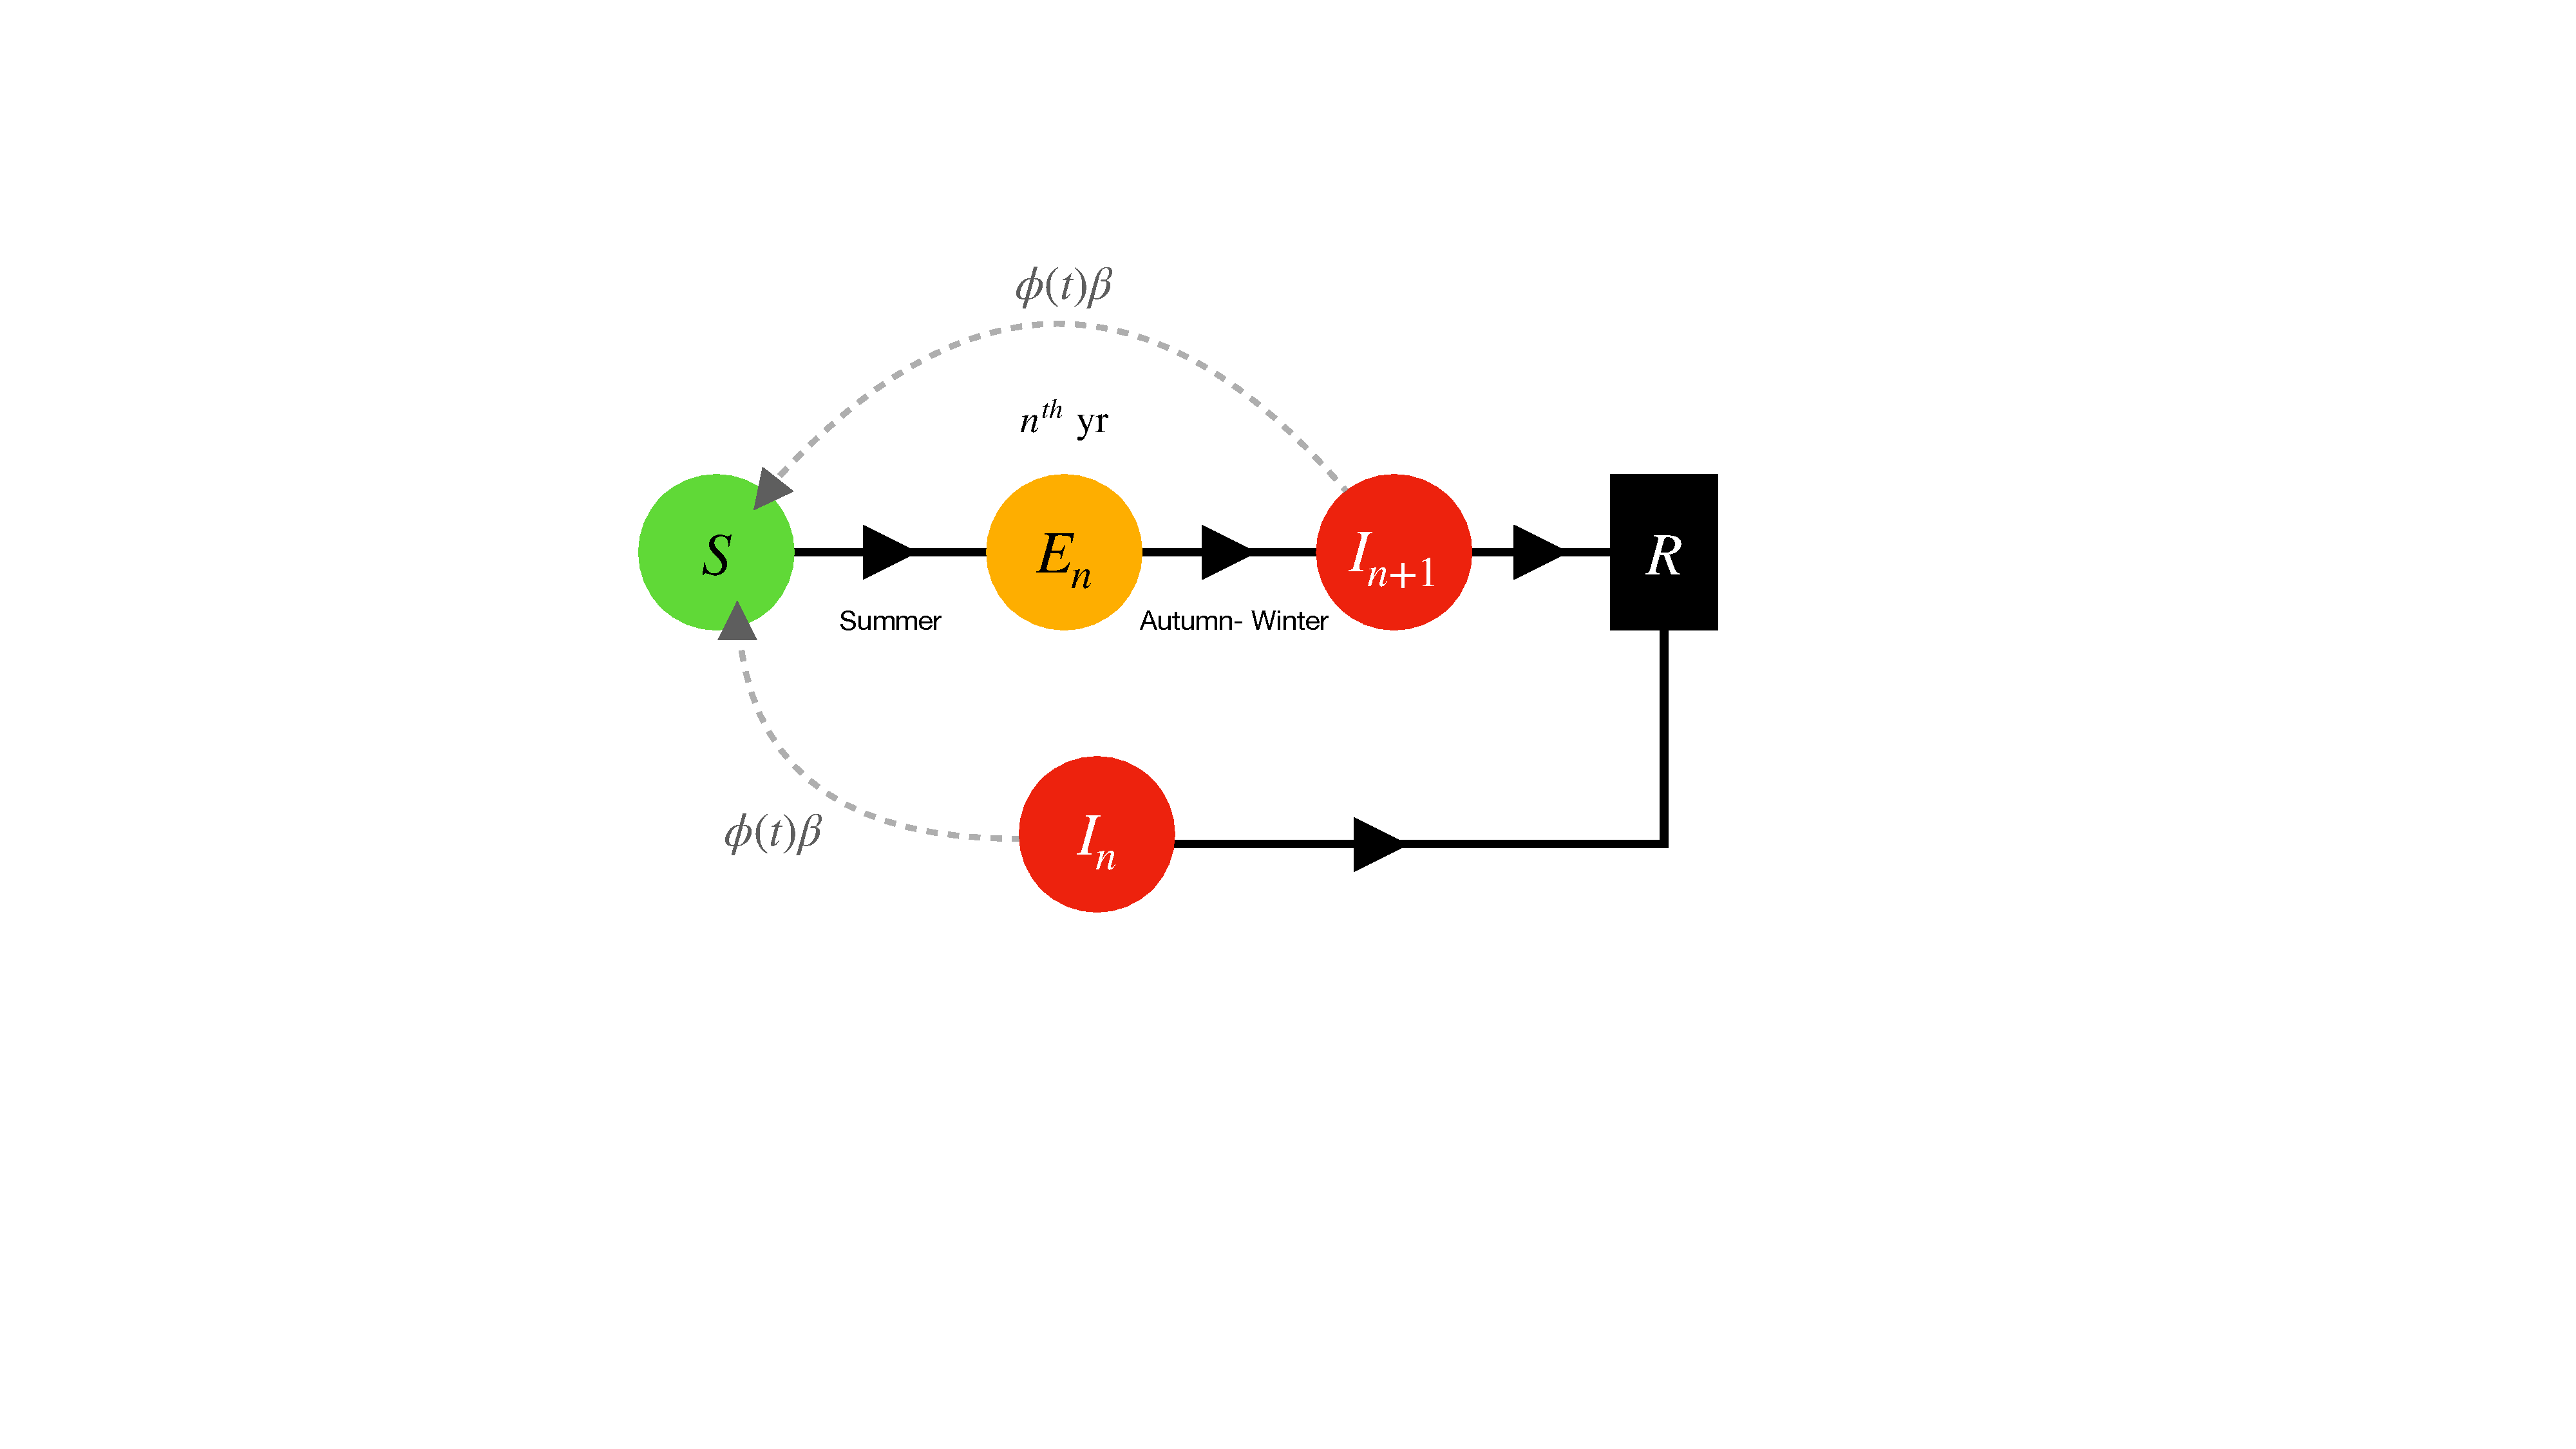
\includegraphics[scale=0.40]{chapter6/figures/fig1-seir-transitions.pdf}
    \caption{The seasonal $SEIR$ model of ADB. (a) In year $n$ of an outbreak, an infectious tree may cause a transition $S\rightarrow E_n$ during summer, depicted by the bottom dashed grey arrow. A tree that becomes latently infected in year $n$ will lead to an infectious tree in year $n+1$. Eventually, all infected ash are removed without the possibility of recovery. (b) The yearly cycle of the pathosystem ADB. Leaf-flush coincides with the sporulation season. Sporulating fruiting bodies release ascospores between June-September. Ash shedding takes place from late summer-early winter. }
    \label{fig:SEIR-transitions}
\end{figure}

Each lattice point in the $L\times L$ domain is chosen to represent a $5\mathrm{m}\times5\mathrm{m}$ patch of land that approximates the canopy cover of an average ash tree
\textemdash although young saplings typically assume less area. 
A domain resolution of $5\mathrm{m}\times5\mathrm{m}$ yields an upper bound of $400$ ash trees per hectare of canopy cover, indicative of some densely populated ash stands \cite{ash-tree2, ash-tree1}. % CHECK!

\subsubsection{Transitions: $S\rightarrow E_n$}

Individual tree-to-tree interactions are modelled as a system of particles\textemdash discussed in chapter \ref{ch5:dispersal-model}.
Transitions from $S$ to $E$ involve two components: a time-varying infectivity $\beta\phi(t)\in [0, 1]$ and dispersal function $D(r; \ell)\in [0, 1]$.
A thin-tailed Gaussian was considered alongside a normalisable fat-tailed inverse power law distribution to model dispersal.

In year $n$, ash located at position $x$ may transition into the exposed category under the influence of infected ash located at $x^\prime$, denoted by $S_x \rightarrow E_{x,n}; I_{x^\prime, n}$.
The probability of transition follows:
\begin{equation}
    Pr(S_{x} \rightarrow E_{x,n} ;\ I_{x^{\prime}, n} ) = \beta  \phi(t) D(r;\ell)
\end{equation}
where $r$ is the distance between $x$ and $x^{\prime}$, and $\phi(t)$ is a time-dependant function reflecting the seasonal life-cycle of ADB, henceforth referred to as the \textit{sporulation function}.
As explained in chapter \ref{ch5:dispersal-model}, transition probabilities are computed for each step a host remains infectious.

\begin{table}
\centering
    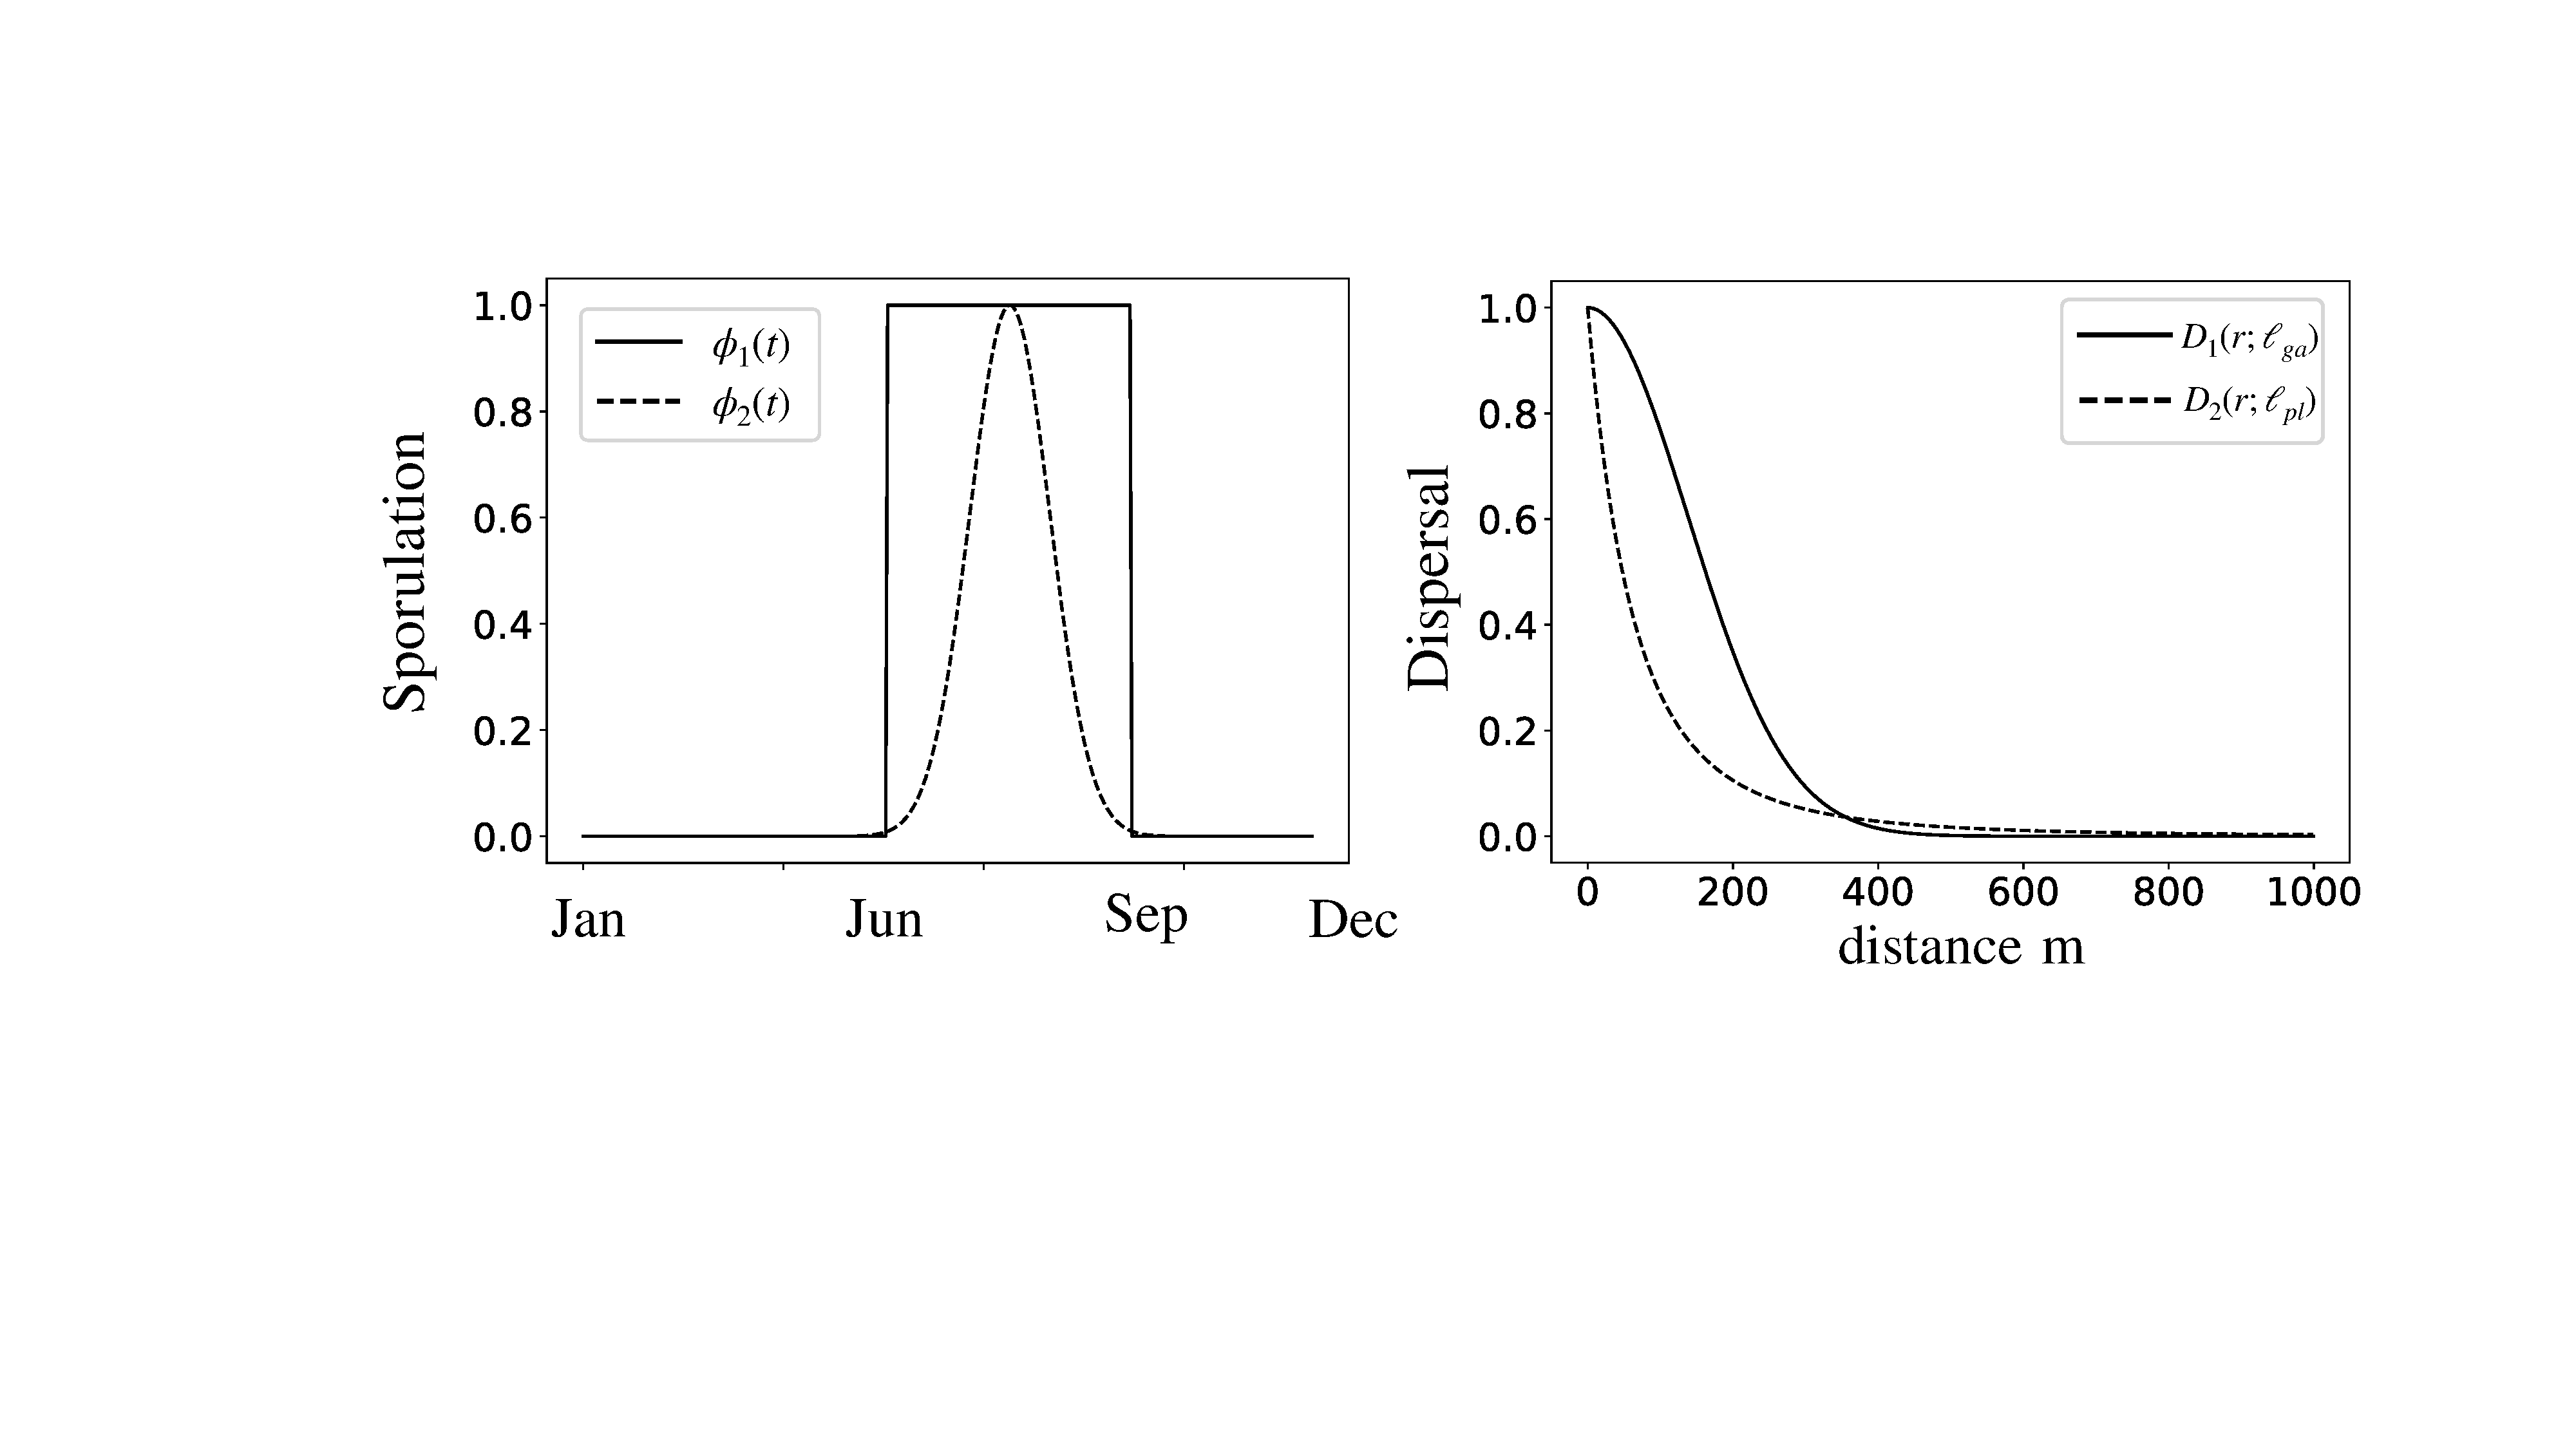
\includegraphics[scale=0.3]{chapter6/figures/fig-phi-disp.pdf}
\begin{tabular}{  p{2.3cm}  p{10cm}  p{3.cm} }
\multicolumn{3}{c}{Infection models} \\
 \hline
 Model name &  $Pr(S_{x} \rightarrow E_{x,n}; I_{x^{\prime}}) \in [0, 1]$ & $\beta^*$ factor\\
 \hline
 1: $\phi_1$-ga & 
 \[= \left\{
\begin{array}{ll}
      \beta  \exp\Big[-\frac{r^2}{\ell^2_{ga}}\Big] &  t \in [\mathrm{June, September}] \\
      0 & \mathrm{otherwise} \\
\end{array} 
\right. \] & $\frac{1}{T} \frac{1}{\pi\ell_{ga}^2}$  \\
 2: $\phi_1$-pl & 
 \[   = \left\{
\begin{array}{ll}
      \beta  \big[1 + \frac{r}{\ell_{pl}}\big]^{-a}  &  t \in [\mathrm{June, September}] \\
      0 & \mathrm{otherwise} \\
\end{array} 
\right. \] & $\frac{1}{T} \frac{(b-1)(b-2)}{2\pi\ell_{pl}^2}$  \\
3: $\phi_2$-ga & 
  \[  =  \beta \exp\Big[-\frac{(t - T_{SP})^2}{2\sigma_{SP}^2}\Big] \exp\Big[-\frac{r^2}{\ell^2_{ga}}\Big]
\]  
  & $ \frac{1}{\sqrt{2\pi}\sigma_{SP}} \frac{1}{\pi\ell_{ga}^2}$ \\
  && \\
4: $\phi_2$-pl & 
  \[ =  \beta \exp\Big[-\frac{(t - T_{SP})^2}{2\sigma_{SP}^2}\Big] \big[1 + \frac{r}{\ell_{pl}}\big]^{-a}
\]  
  & $ \frac{1}{\sqrt{2\pi}\sigma_{SP}} \frac{(b-1)(b-2)}{2\pi\ell_{pl}^2}$ \\
   && \\
 \hline
 \end{tabular}
  \caption{Four infection models are considered, composed of either: Gaussian (ga) or inverse power law (pl) dispersal, and step function ($\phi_1$) or peaked ($\phi_2$) sporulation. All component functions yield values in the interval $[0, 1]$ and are normalisable. The corresponding model parameters are shown below in Table \ref{tab:SEIR-model}. 
  The left-hand column shows the normalisation factor used to construct $\beta^*$, i.e. to fix epidemic-impact between models.}
\label{tab:model-variants}
\end{table}

\begin{table}[h]
\centering
\begin{tabular}{l l l}
\hline
\textbf{Model parameter} & \textbf{Description} & \textbf{Value(s) taken}\\
\hline
$\rho$  & Tree density & $0.00 - 0.10$ \\ 
$\beta$ & Infectivity & $0 - 10^{-3}$ \\
$\ell_{ga}$ & Gaussian scale parameter $=\sqrt{2}\sigma_{ga}$ & $196\mathrm{m}$ \\
$\ell_{pl}$ & inverse power law scale parameter & $203\mathrm{m}$ \\
$a$ & Inverse power law exponent & $3.3$ \\
$t$ & Time-step & $1\ \mathrm{day}$\\
$T$ & Days in Sporulation peak June - September & 122  \\
$T_{SP}$ & Peak sporulation $\phi_2$ & end of July \\
$T_{LS}$ & Peak ash leaf-shedding & mid-November \\
$\alpha$ & Lattice constant & $5\mathrm{m}$ \\
$L$ & Lattice dimension (i.e. an $L\times L$ patch)  & $200$ - $2000$ \\
$A$ & Domain area (defined by $\alpha L\times \alpha L$) & $1\mathrm{km^2}$ - $20\mathrm{km^2}$ \\
$\lambda$ & Mean infectious life-time & $5\ \mathrm{years}$ \\
$R_0$ & Mean reproduction number & $0-20$ \\
\hline
\end{tabular}
\caption{Parameters used in the $SEIR$ model of ash dieback. The dispersal parameters are taken from \cite{grosdidier2018tracking} and the typical tree densities of ash are informed from by \cite{hill.data}.}
\label{tab:SEIR-model}
\end{table}

The sporulation function $\phi$ dictates when infectious trees in $I_n$ produce new secondary infections. 
For ADB, sexual reproduction repeats yearly from June to September during its \textit{`sporulation season'}.
As such, $\phi$ is non-zero during the sporulation period.
Two sporulation functions are considered, $\phi_1$ and $\phi_2$, based on the step function and normal distribution, respectively.
Sporulation is the topic of section \ref{ch6:sporulation} below, alongside the precise functional form of $\phi_1$ and $\phi_2$.
Altogether there are four infection models, summarised in table \ref{tab:model-variants}.

Once in the $E$ compartment, trees are infected but not infectious, i.e. latently infected.
For example, ash infected with \textit{H. fraxineus} take approximately two weeks to display symptoms \cite{https://doi.org/10.1111/ppa.12048, https://doi.org/10.1111/ppa.12844},
and start to shed infectious leaves in following autumn after infection \cite{gross2014h}.
The compartments $(E_1, E_n,..,E_n)$ represent the same biological state of latently infected, the index $n$ is merely included for convenience to highlight the fact that in this model, it takes latently infected ash takes approximately one year to start producing new secondary infections during the $(n+1)^{th}$ sporulation peak.

\subsubsection{Transitions: $E_n\rightarrow I_{n+1}$}

As defined here, latently infected ash in $E_n$ transitions into the infectious compartment, $I_{n+1}$, at the first onset of seasonal leaf shedding between autumn and winter.
Infected ash disperse infectious leaf litter each year following infection until its eventual demise;
this dynamic assumes that all ash are susceptible and that leaf infection spreads to the ash xylem with perfect fidelity. 
In reality, a variety of genetic and environmental factors determine the ability of ADB to invade an ash\footnote{
The pathogen \textit{H. fraxineus} can infect ash leaves regardless of tolerance. However, only the minority of tolerant individuals can prevent inoculum from spreading to the xylem.}.

A Gaussian distribution represents the onset of ash leaf-shed, and therefore the transition $E_n\rightarrow I_{n+1}$.
The distribution is centred in November, $T_{LS},$ with a two-week standard deviation $\sigma_{LS}$.
Centring the normal distribution in mid-November, with a two-week standard deviation, ensures that the earliest possible onset of leaf-shed (described by the left-hand tail) begins in September.
In the field, the timing of ash shedding their leaves is more complicated and depends on tree age. 
Observations by \cite{hietala2013invasive} suggest that younger ash begin to defoliate in late August, while large dominant ash starts to shed in early October.

Despite a thorough search, litter-fall rates for ash appear to be unknown, so choosing a normal distribution centred in mid-November with a two-week standard deviation is ultimately ill-informed.
Notwithstanding, the normally distributed form of leaf-shedding is supported by observations of leaf litter-fall in deciduous forest \cite{zhang2014seasonal, dixon1976analysis}, 
which typically follow peaked distributions that repeat yearly.
Moreover, research conducted on wetland forests in South Carolina has demonstrated that the temporal pattern of litter-fall peaks yearly between August and November, albeit with some variation \cite{shure1985litter}.
That said, within the $SEIR$ model a the time delay exists between transition $E_n \rightarrow I_{n+1}$ in autumn/winter and the sporulation function $\phi(t)$ becoming sufficiently large in summer;
so we can afford some degree of flexibility in the exact time scale.
From a mathematical standpoint, provided that latently infected ash transitions into the infected compartment before the sporulation season,
the epidemic spread in this model will remain the same.

% The seasonal pattern of litter-fall plays an important role in ecosystem function and forest health. 
% taking into account more involved leaf-shed dynamics
% A more complex model of ADB, involving soil-borne interactions, could incorporate the build up infected leaf biomass into a time-varying $\beta$. 
% However, it remains to be seen if this is necessary to capture the essential dynamics of wind-borne dispersal.

\subsubsection{Transitions: $I_n\rightarrow R$}

The last transition to consider is from infected to removed $I_{n}\rightarrow R$. Given a $95\%$ mortality rate, ADB can be regarded as lethal \cite{ash-dieback-costs}.
Therefore, once an ash tree becomes infected, an eventual transition to the $R$ compartment is assumed with certainty.
As mentioned above, the picture is more complex in reality. 
For example, stress-free trees in urban settings can survive for long periods if pruned \cite{marciulyniene2017can}, and a low minority of healthy tolerant trees can fight off the infection.
Additionally, other edge-cases can contradict this assumption;
laboratory experiments have shown that after a \textit{`massive ascospore inoculation'}, leaf-shed can result before the infection has the chance to spread throughout the tree \cite{https://doi.org/10.1111/mpp.12073}.

Ash dieback affects trees of all ages, with younger ash being more susceptible while larger, mature ash appear more tolerant. 
As a first approximation, infected ash trees were chosen to have exponentially distributed lifetimes with a mean of five years, see table \ref{tab:SEIR-model}.
Experimental observations of ash mortality after years of infection support this decision. 
In particular, reports of $5\%$ mortality after two years of infection \cite{kessler2012dieback}, $75\%$ mortality within five years \cite{langer2015ash}  % Brush up in relation t age classes
and no observations of infected ash surviving beyond $15$ years \cite{wylder2018evidence} provide some guidance towards an approximate time-scale.
The precise probability distribution describing $I_{n}\rightarrow R$ is, to my knowledge, non-existent in the literature.

\subsection{Dispersal parameterisation}

Dispersal was informed by data collected in France by \cite{grosdidier2018tracking}.
The experiment conducted by \cite{grosdidier2018tracking} tracked ADB ascospores about known sources of infection\textemdash reviewed in chapter \ref{chapter2:litreview}.
The authors considered a Gaussian and inverse power law kernel of the form:
\begin{equation}
    Pr(a, r) = \frac{1}{\pi \ell_{ga}^2} \exp\big[-\frac{r^2}{\ell_{ga}^2}\big]
\end{equation}
and
\begin{equation}
    Pr(a, r) = \frac{(b-1)(b-2)}{2\pi \ell_{pl}^2} \big[ 1+ \frac{r}{\ell_{pl}}\big]^{-b}
\end{equation}

where parameters $\ell_{ga}$ and ($\ell_{pl},\ b$) are given in table \ref{tab:SEIR-model}.
Notably, the researchers measured dispersal parameters at local and regional spatial scales, between $[0 \sim 1\mathrm{km}]$ and $[10 \sim 100 \mathrm{km}]$ respectively.
Given that the $SEIR$ model is small-scale, the local-scale values were used to parameterise dispersal in the $SEIR$ model.

Dispersal data collected by \cite{grosdidier2018tracking} relate to a French landscape and environmental conditions.
Therefore, parameterising dispersal with these parameters assumes that the spread of ADB in GB is comparable to ADB spread in France. 
Nonetheless, a noticeable difference in the French climate, landscape and, importantly, wind patterns would lead to some differences in ADB dispersal patterns in GB.
Notwithstanding these differences, it stands to reason that dispersal parameters, if measured over a smaller, local spatial scale, would be less pronounced in both landscapes. 

Lastly, the regional-scale dispersal analysed by \cite{grosdidier2018tracking}, measured over spatial scales of $10$-$100\ \mathrm{km}$, is thought to contain artefacts of LDD by human-mediated transport.
The regional-scale spread of ADB though LDD on the order of $10-100\mathrm{km}$ is beyond the scope of the present chapter.

\subsection{Normalising $\beta$ between models}

Undesirably, the scale of $\beta$ varies between model variants, due to the difference in area under the curves of $\phi_1$, $\phi_2$, $D_1$ and $D_2$.
Similarly, this behaviour was witnessed in chapter \ref{ch5:dispersal-model} when the NLM was simulated with different dispersal length scales.
To constrain each model on the same $\beta$-axis, the appropriate normalisation constant (shown in Table \ref{tab:model-variants}) is once again factored out of the infectivity probability $\beta$ 
e.g. for $\phi_1$-ga, this takes the form: 
\begin{equation}
    \beta = \frac{\beta^*}{T \pi \ell^2_{ga}} \in [0, 1]
\label{eq:normalised-beta}
\end{equation}
where $\beta^*$ is an auxiliary parameter that does not depend on the form of sporulation or dispersal function (provided that both functions are normalisable);
hence, as before, $\beta^*$ isolates infection pressure to a single parameter.
On account of the sporulation function and longer range kernel, $\beta^*$ in equation \ref{eq:normalised-beta} assumes a larger value when compared to $\beta^*$ in chapter \ref{ch5:dispersal-model}.


\begin{landscape}
\begin{figure}
    \centering
    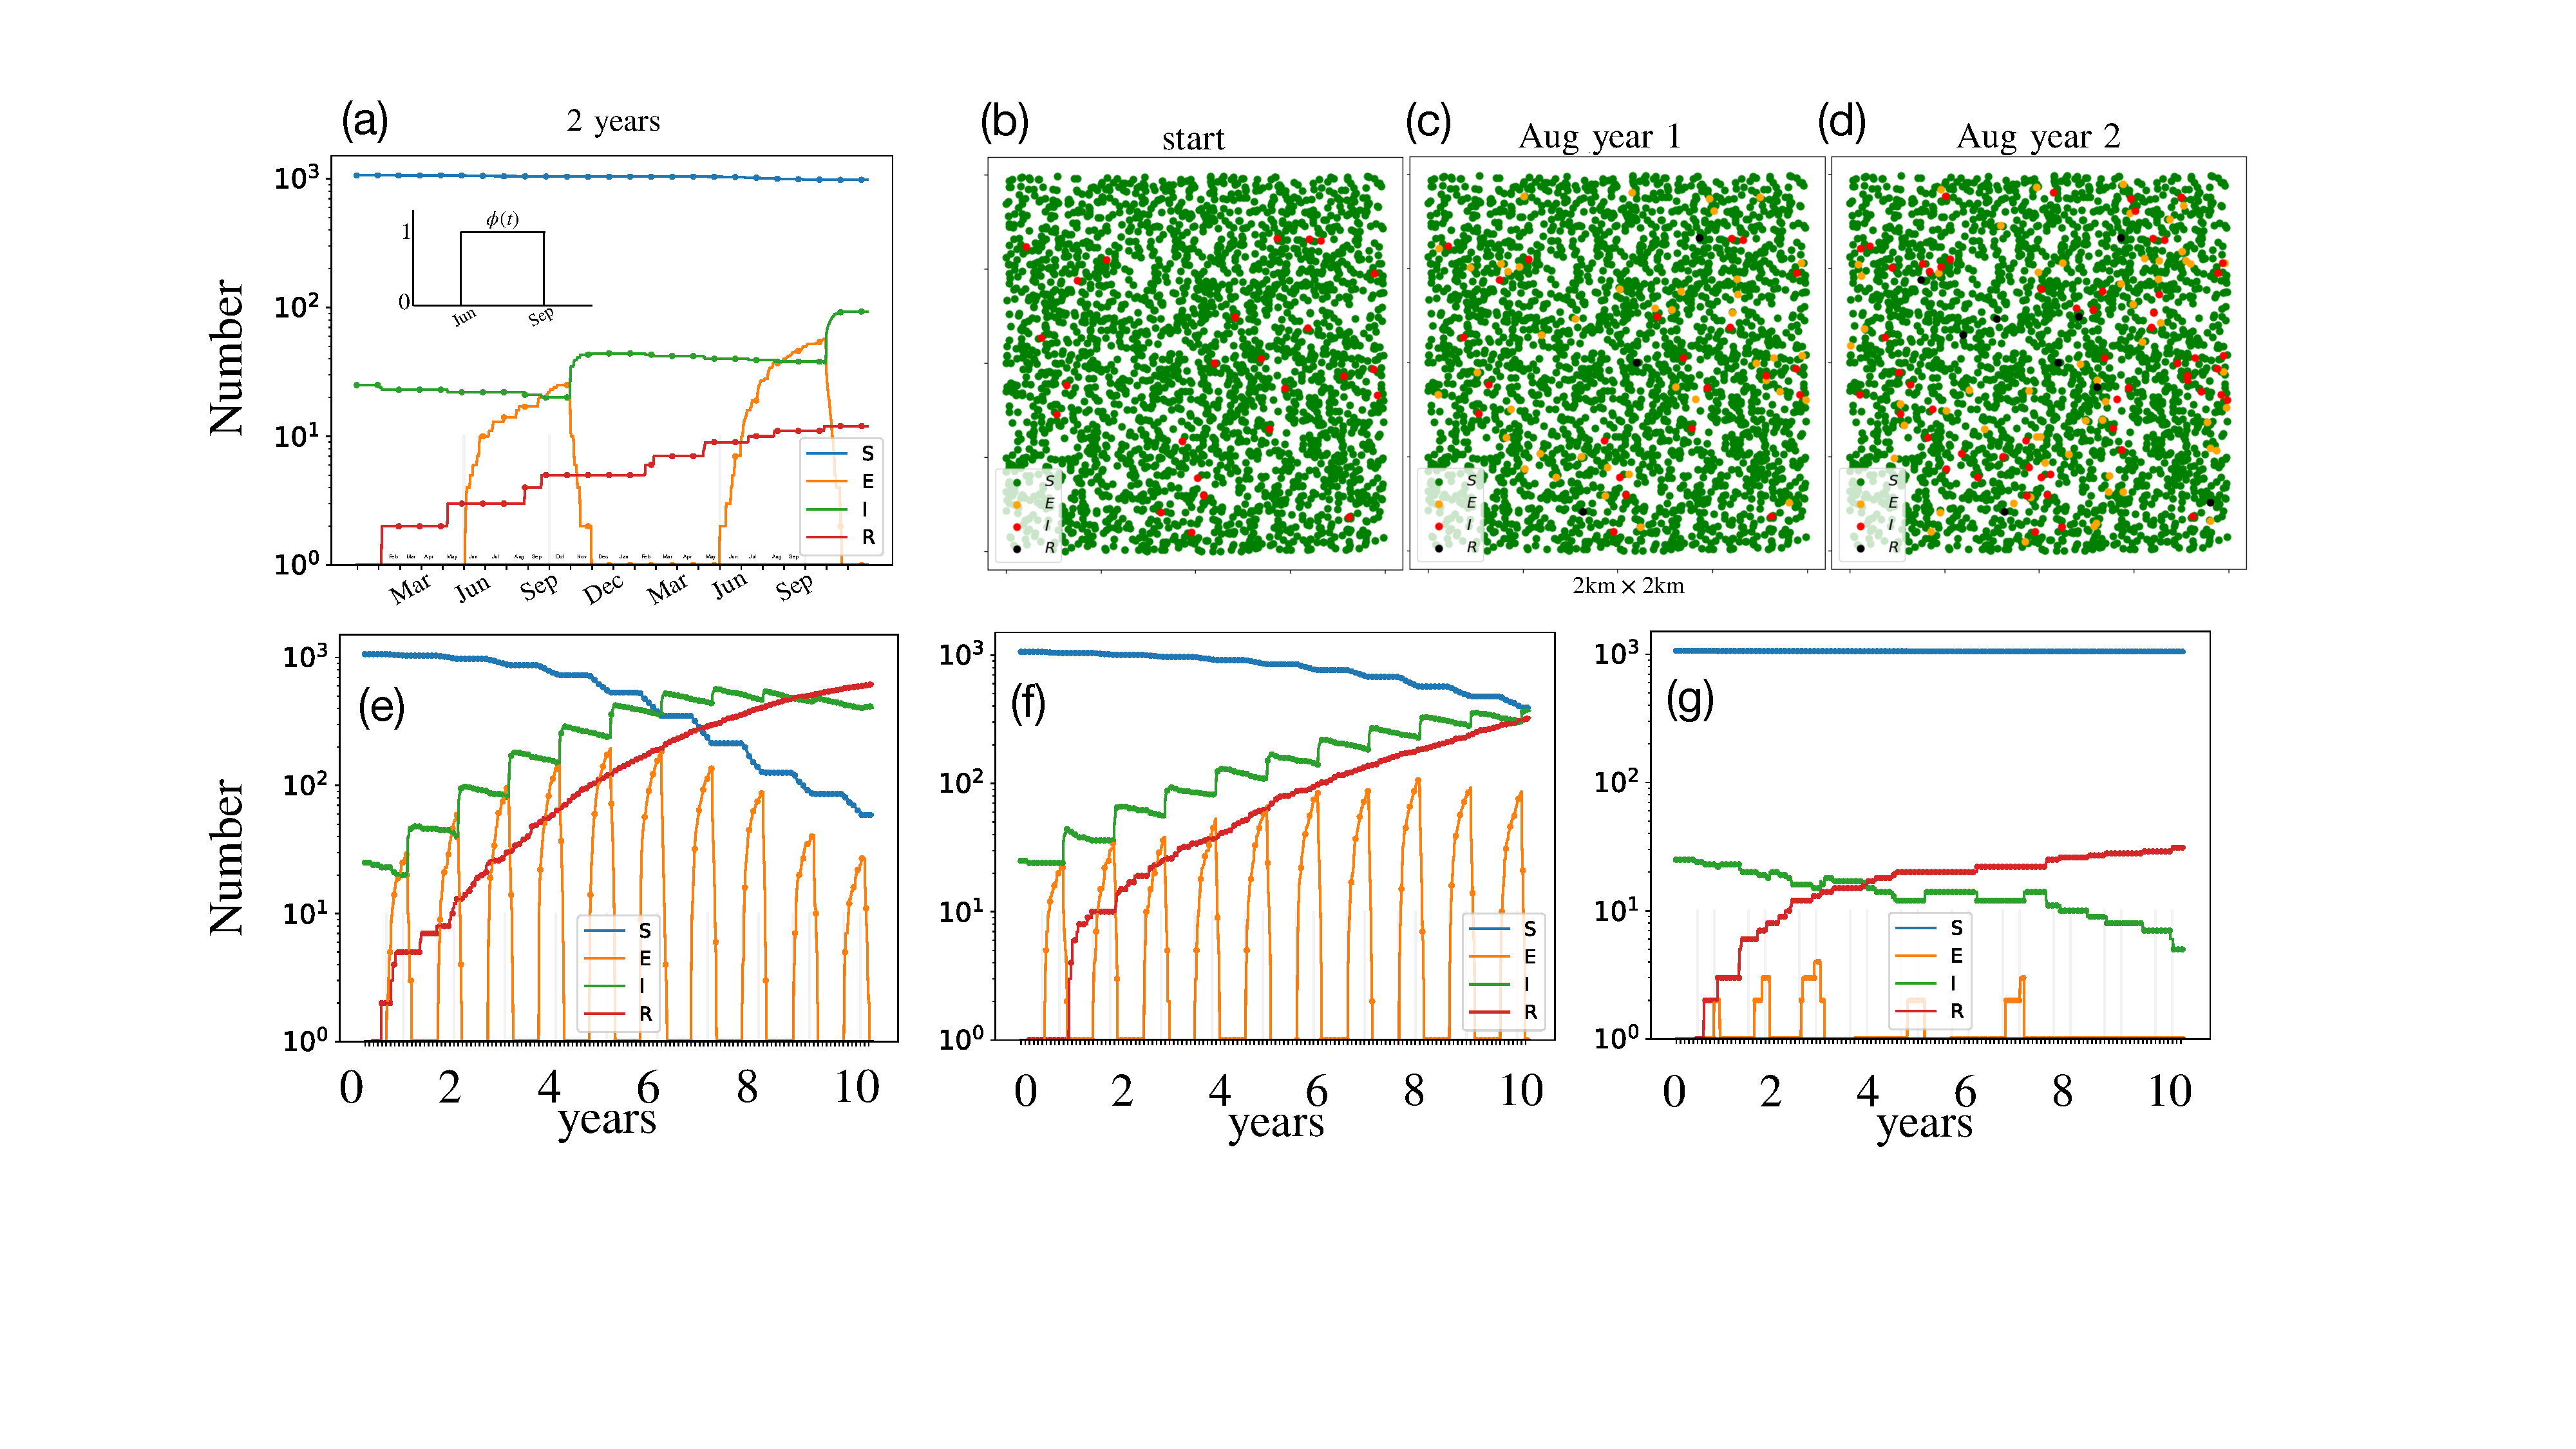
\includegraphics[scale=0.45]{chapter6/figures/fig4-seir.pdf} % SHOW 5 YEAR simulations instead, 10 years is too long...
     \caption{Simulating the $SEIR$ model over the median ash density, i.e. $\rho_{\mathrm{med}} = 0.011$. 
     In all panels, a small clump of $20$ infected hosts seeds the domain centre at time $t=0$.
     (a-b) The number of ash in each $SEIR$ compartment is plotted over five years for the model $\phi_1$-ga.
     Panels (a) and (b) depict simulations above ($\beta^*=2000$) and below ($\beta^*=500$) the epidemic threshold, respectively. 
     (c-f) The spatial progression of disease in a $2\mathrm{km} \times 2\mathrm{km}$ domain over a full year for model $\phi_1$-pl; 
     infectivity is fixed to  $\beta^*=3000$, well above the threshold.
     From the first sporulation season (c)-(d) to the second (e)-(f), secondary infections scatter throughout the whole domain, in contrast to the wave-like behaviour witnessed for small dispersal length scales in chapter \ref{ch5:dispersal-model}.}
    \label{fig:SEIR-spread}
\end{figure}
\end{landscape}


\section{Seasonal $SEIR$ model behaviour}
\label{sec:seir-behaviour}

The essential $SEIR$ model behaviour is shown in Figure \ref{fig:SEIR-spread}, simulated with the median ash density in Great Britain\textemdash according to \cite{hill.data}.
For each year after the outbreak, a rise in the number of latently infected ash in $E$ can be seen during summertime sporulation, June-September, followed by a rise in the number of infectious ash in the autumn-winter. 
All model variants display the same pattern of seasonal behaviour. 

The number of ash in the $SEIR$ compartments is shown in Figure \ref{fig:SEIR-spread}(a-b) for two infectivity parameters in a $1\mathrm{km}\times1\mathrm{km}$ domain.
Figures \ref{fig:SEIR-spread}(a-b) depict two scenarios above and below the epidemic threshold for model $\phi_1$-ga;
the compartments are plotted over $5$ years with infectivity ($\beta^*$) parameters shown. 
In Figure \ref{fig:SEIR-spread}(a), the number of ash in $S$ decline, shown by the green line,
and during seasonal sporulation, large spikes in the number of latently infected ash can be seen in orange. 
Then, latently infected ash transition into $I$ during autumn and winter, as shown by the seasonal rise of $I$ in green.
For infectivity parameters below the epidemic threshold, Figure \ref{fig:SEIR-spread}(b), $S$ remains approximately constant as $I$ slowly declines. 
Interestingly, Figure \ref{fig:SEIR-spread}(b) demonstrates persistence in model of ADB; 
whereby, even if the epidemic parameters are below the threshold, the fungus may survive for long periods. 
In general, persistence in plant-based pathogens is one aspect that complicates epidemic control\textemdash see chapter \ref{ch3:invasions_and_persistence} for a review of invasion and persistence in the spread of plant-based diseases.

The spatial progression of ADB in the $SEIR$ model is shown in Figures \ref{fig:SEIR-spread}(c-f) over a full year. 
The simulation in Figure \ref{fig:SEIR-spread}(c) begins with an initial condition of $20$ infected ash centrally distributed in the host landscape during March (not shown). 
At this point in the year, fungal fruiting bodies on infected leaf litter will be preparing to release ascospores.
During sporulation, secondary infections are produced, and latently infected ash spread throughout the domain, depicted by the orange dots in Figure \ref{fig:SEIR-spread}(c-d). 
At any time step, the chance of removal to the $R$ compartment s non-zero, demonstrated by the small number of black dots in Figures \ref{fig:SEIR-spread}(c-d).
After the sporulation season ends in September (not shown), latently infected ash begin to transition into the $I$ compartment;
eventually, all latently infect ash become infectious during the following season, reflected by the increased number of red dots in Figure \ref{fig:SEIR-spread}(e). 
The cycle will continue when the next cohort of secondary infections are produced in the following summer when the sporulation function next becomes non-zero.

\subsection{Sporulation: time-varying infectivity}
\label{ch6:sporulation}

Time varying infectivity rates are an important concept in epidemiology, this is true of epidemics in both human/animal \cite{svensson2007note, liu2012infectious} 
and botanical populations \cite{suffert2018some, leclerc2014estimating, time-varying-infectivity}.
In particular, ADB is known to have a seasonal life-cycle, and time-varying infectivity \cite{grosdidier2018tracking, hietala2013invasive}. 
The peak of ADB infectivity occurs during summertime sporulation when fruiting bodies on shed litterfall release ascospores.

To demonstrate robustness in the approach, two sporulation functions, $\phi_1(t)$ and $\phi_2(t)$, are used to model the time-dependent ADB ascospore production.
The choice of sporulation functions were inspired by the modelling work of \cite{time-varying-infectivity} and \cite{segarra2001epidemic}
(reviewed in chapter \ref{ch2:lit-rev-compartmentalised-models}). 
Sporulation functions are described by step function and a normal distribution located at the midpoint between June and September:

\begin{equation}
\phi_1(t)  = \left\{
\begin{array}{ll}
      1 &  t \in [\mathrm{June,\ September}] \\
      0 & \mathrm{Otherwise} \\
\end{array} 
\right.
\end{equation}
and 
\begin{equation}
     \phi_2(t) =  \exp\big[-\frac{(t - T_{SP})^2}{2\sigma_{SP}^2}\big]
\end{equation}

\begin{figure}.
    \centering
    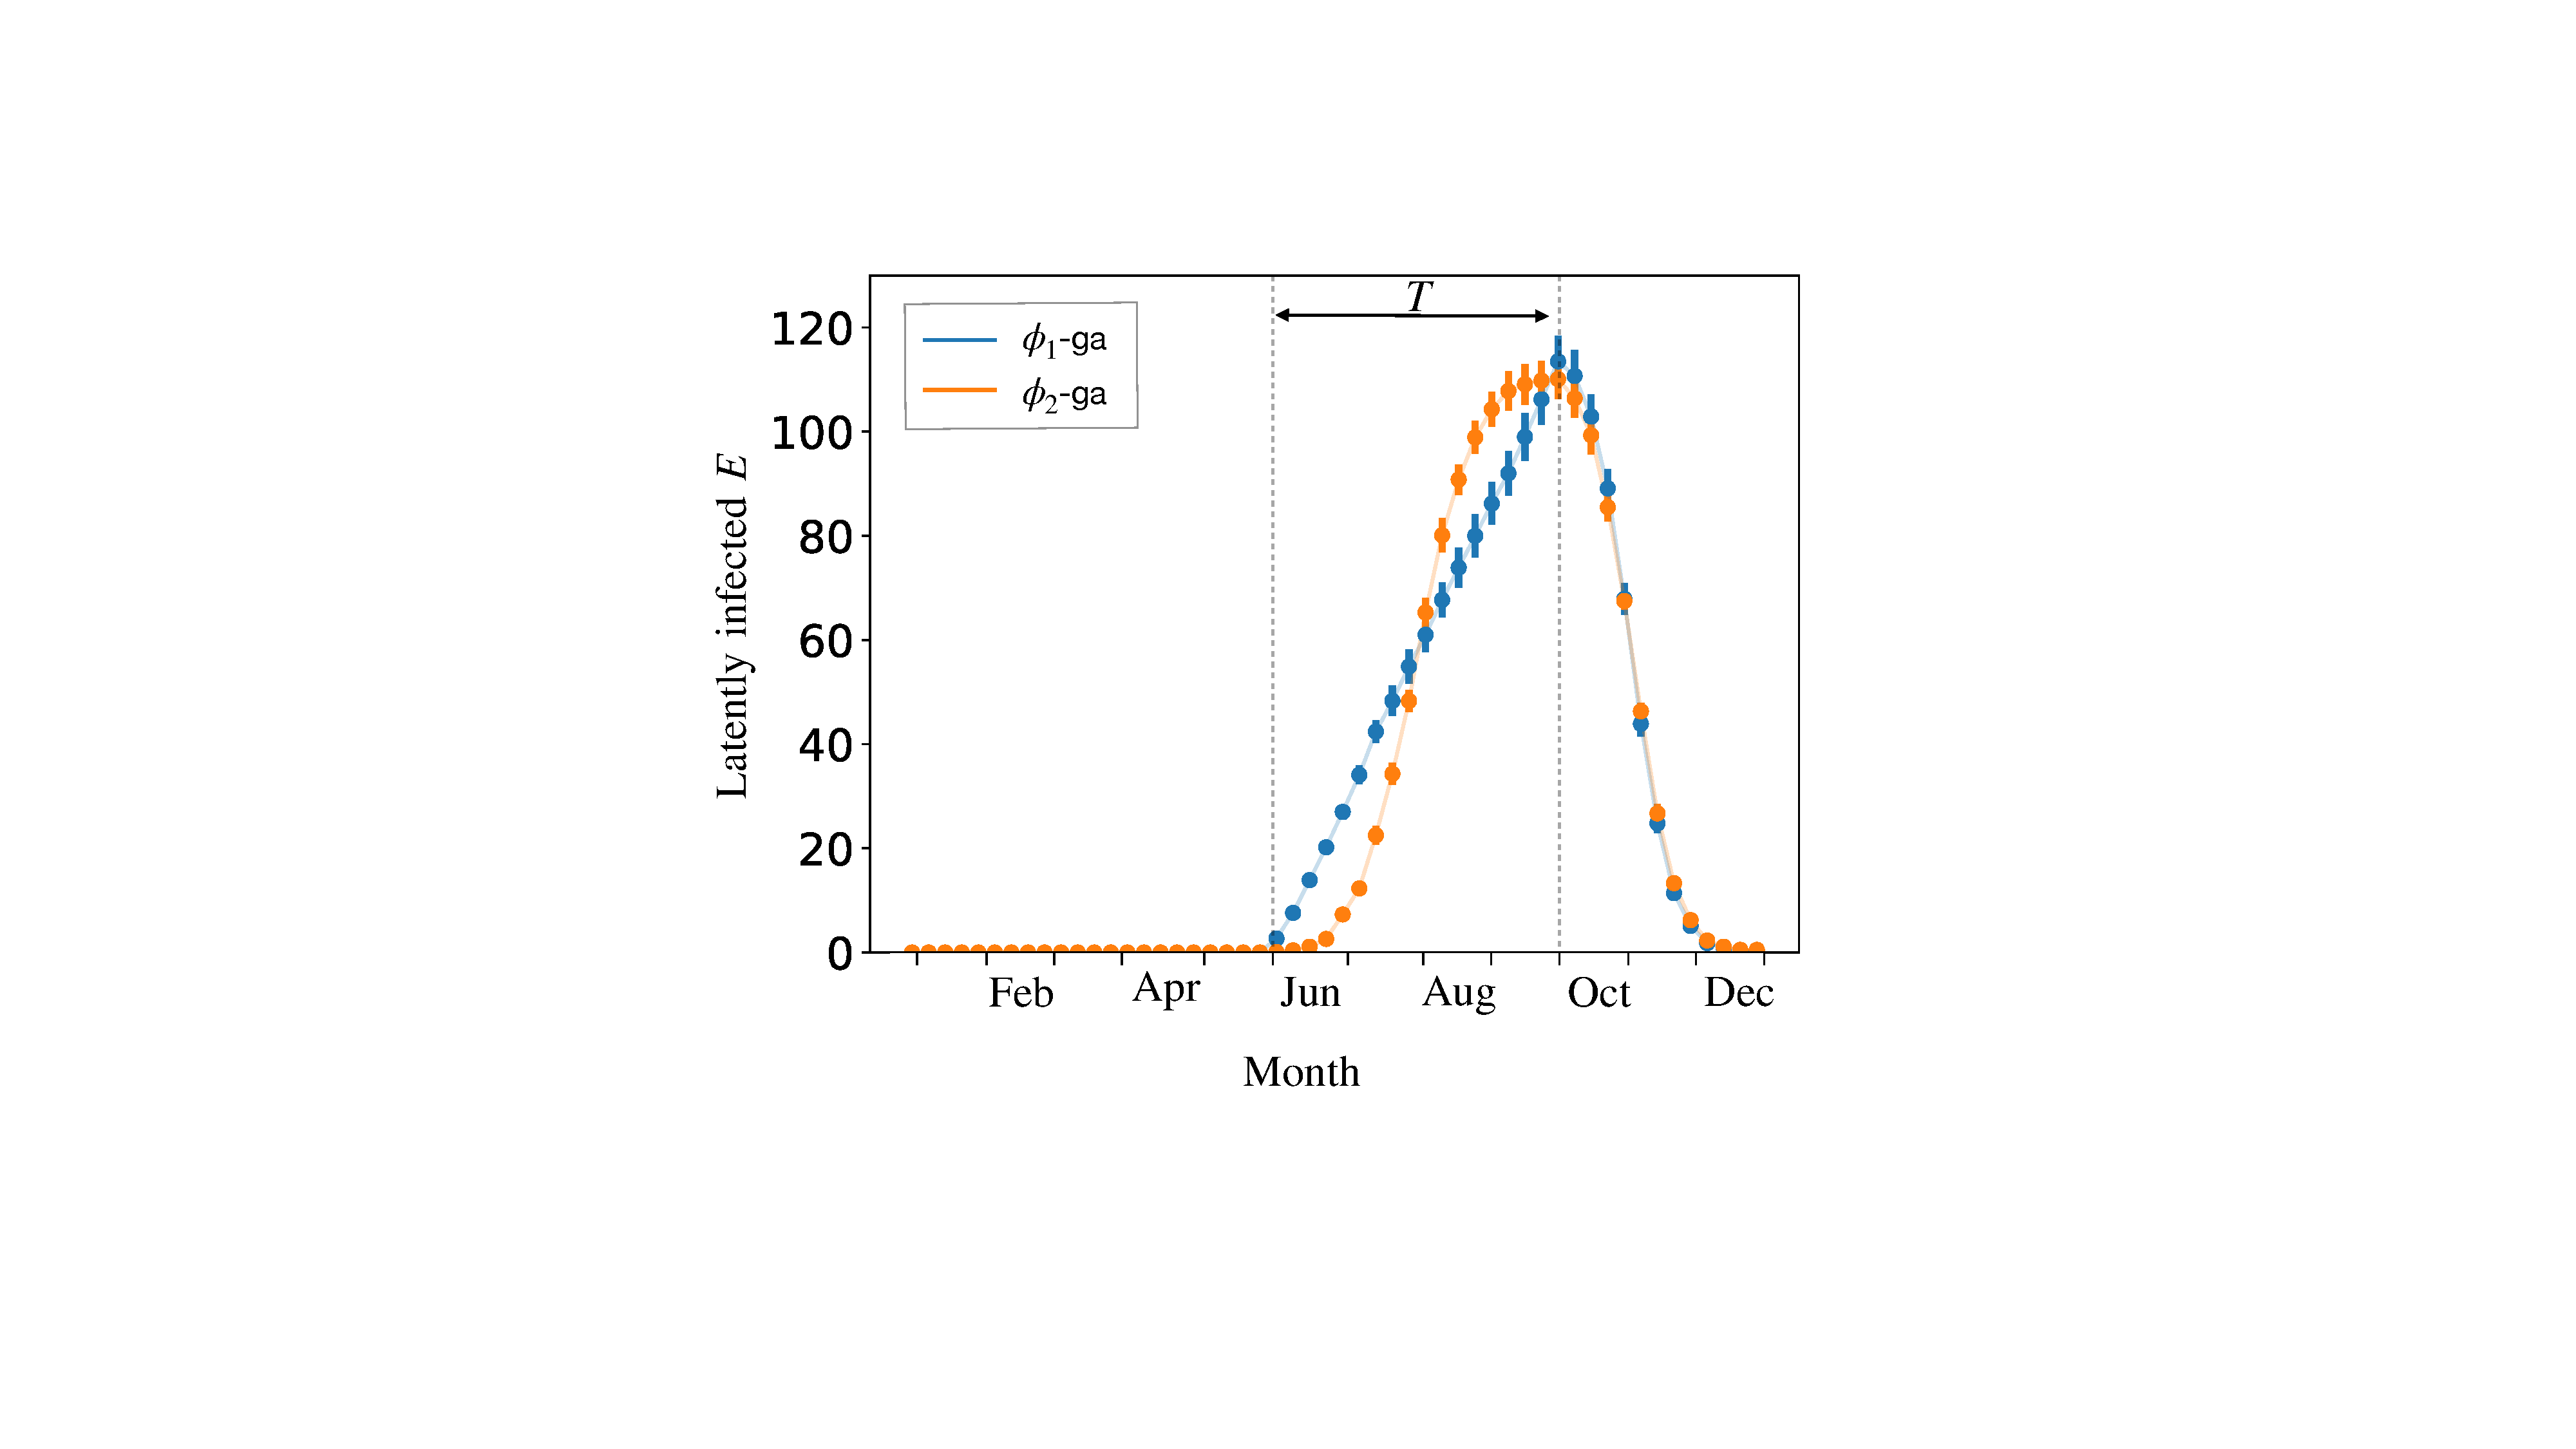
\includegraphics[scale=0.35]{chapter6/figures/fig5-sporulation.pdf}
    \caption{One year simulations contrasting the form of sporulation for models $\phi_1(t)$-ga and $\phi_2(t)$-ga, (a) and (b) respectively. 
    Both (a) and (b) depict the average number of infected trees that transition into the $E$ compartment over a single sporulation season; the standard error is shown by the error bars.
    An auxiliary infectivity, of value $\beta^*=2000$, effectively matches the epidemic impact between models\textemdash indicative of the area under each curve.}
    \label{fig:SEIR-sporulation}
\end{figure}

where $T_{SP}$ is taken to be the mid-point of June-September (i.e. late July/early August) and $\sigma_{SP}^2$ is a standard deviation of two weeks.
As discussed above, the choice of sporulation peak $T_{SP}$ and standard deviation $\sigma_{SP}$ together inform the earliest transitions $S\rightarrow E$ for $\phi_2$.
Due to the seasonality and perennial nature of ADB, both $\phi_1(t)$ and $\phi_2(t)$ repeat yearly, becoming non-zero during the months of June and September\footnote{Variations in ADB sporulation have been noted between European countries \cite{https://doi.org/10.1111/mpp.12073}, along with the potential for early-onset sporulation in the face of favourable environmental conditions. Although, the most generally agreed upon sporulation period is thought to be from June to September.}.
For $\phi_2$, the chance of new secondary infections outside of June-September is trivially small.

Figure \ref{fig:SEIR-sporulation} contrasts sporulation models by computing the number of ash transitioning into the $E$ compartment for one season over an ensemble of size $10$.
Simulations started with $100$ infected ash distributed randomly throughout a $\mathrm{5km \times 5km}$ domain at the mean GB ash density in January (i.e. time $t=0$ ).
Both models show a rise in the number of infected ash during the sporulation season.
The infectivity rate for function $\phi_2$ can be seen to vary, in contrast $\phi_1$ is uniform\textemdash both dispersal models $\phi_1$-pl and $\phi_2$-pl demonstrated the exact behaviour.
Although infectivity rates differed, the normalised infectivity $\beta^*$ ensured the same approximate area under each curve and, therefore, epidemic impact.

Both $\phi_1(t)$ and $\phi_2(t)$ aim to mirror the seasonal time-dependence of \textit{H. fraxineus} sexual reproduction.
In the seasonal $SEIR$ model, time-varying infectivity is achieved by multiplying the infectivity parameter with a sporulation function $\beta\phi(t)$.
In line with the parsimonious approach undertaken thus far, $\phi_1(t)$ and $\phi_2(t)$ are generic and aim to capture the essential dynamics of ADB spread.
However, a more complex model could aim to fit $\phi(t)$ to spore-trapping data, which could resemble a Gaussian-k function (e.g. see Figure 2. in \cite{grosdidier2018tracking}).
Although different sporulation models lead to the same effective behaviour (as discussed more below in section \ref{sec:tree-mortality}), 
non-uniform infectivity rates for ADB have a more robust basis in the literature \cite{grosdidier2018tracking, time-varying-infectivity, hietala2013invasive, segarra2001epidemic}.
So, the function $\phi_2$ can be considered more representative due to the non-uniformity and infectivity peak.

\subsection{Tree mortality}
\label{sec:tree-mortality}

Ash mortality due to ADB has been well-researched in different European countries, frequently over long-running 10-20 year experiments.
In this section, tree mortality is studied over long time scales to give insight into the scale of the epidemic, pathogen invasiveness and domain sensitivity.
However, host demography was neglected from the model, which is desirable for modelling the spread of pathogens targeting long-lived hosts \cite{doi:10.1098/rstb.1996.0059}.
Therefore, the long-running simulations presented in this section approximate the spread of ADB over considerable time scales to first-order.

\begin{figure}
    \centering
    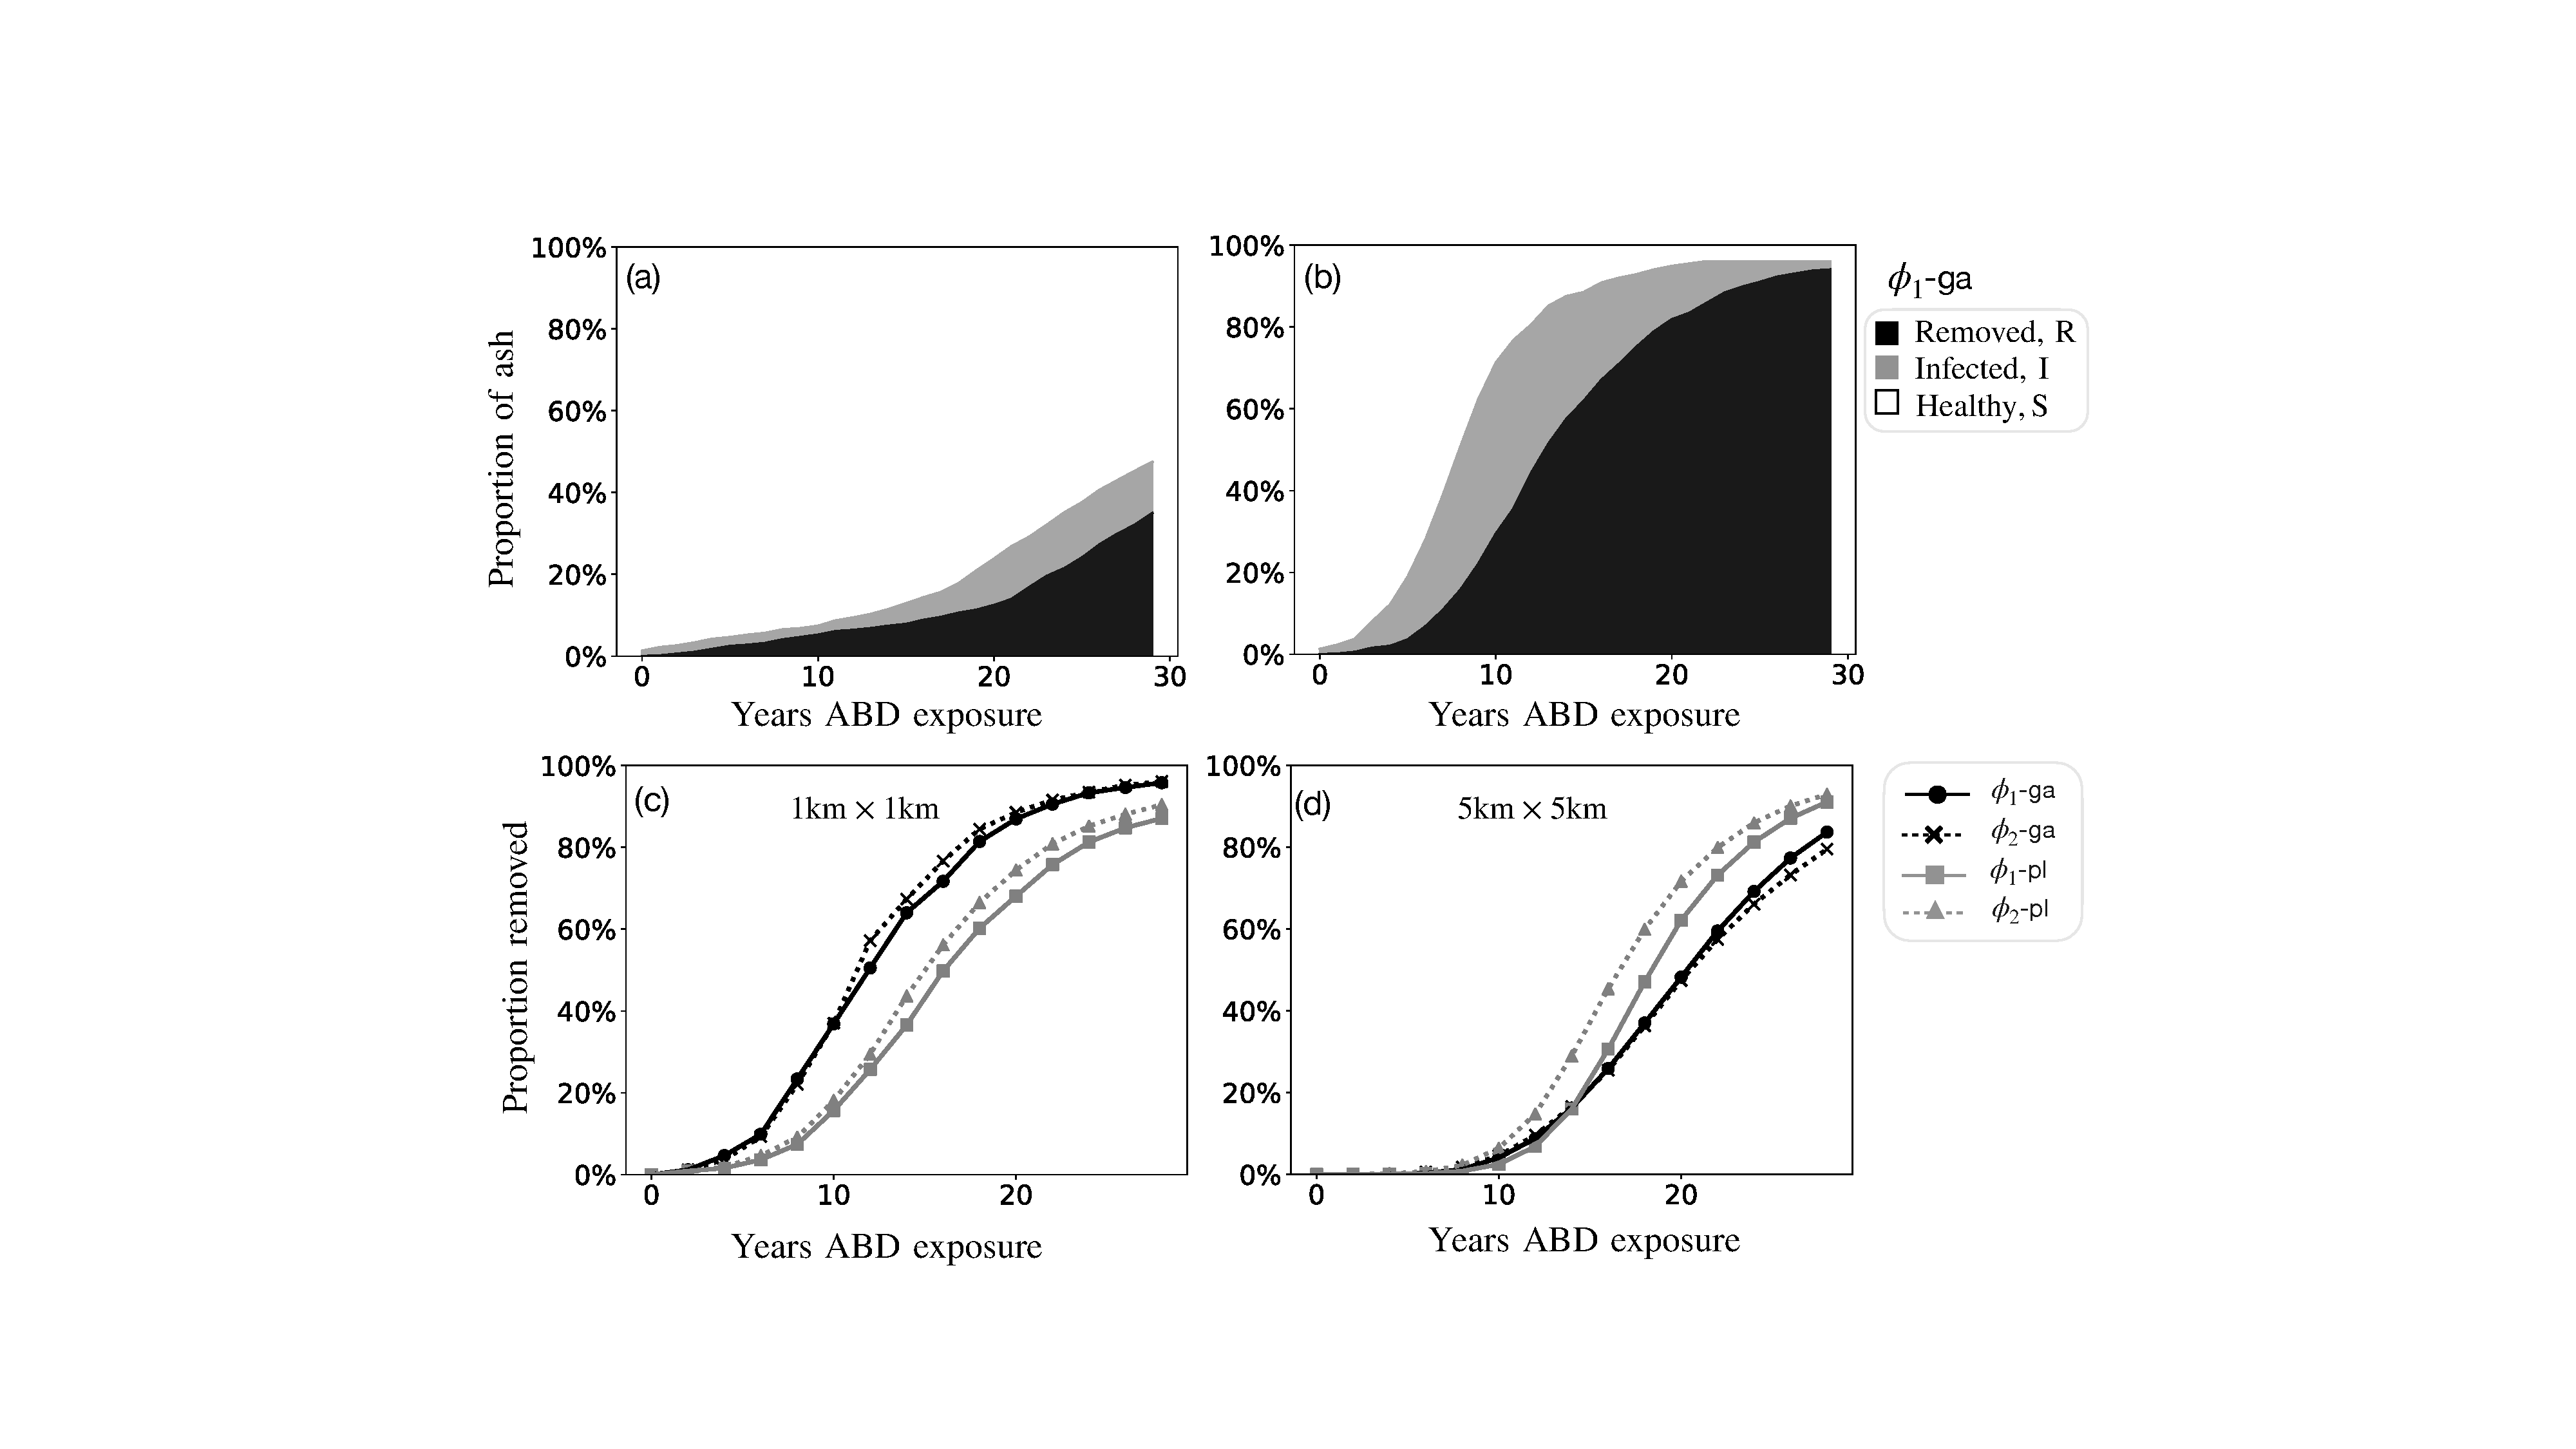
\includegraphics[scale=0.42]{chapter6/figures/fig6-mortality.pdf}
    \caption{Epidemic-scale in the $SEIR$ model, as measured by the proportion of ash in $S$, $I$ and $R$ (a-b) The proportion of ash in $S$, $I$ and $R$ is shown over $10$ years of ADB exposure for $\phi_1$-ga. Two different values of infectivity, $\beta^*=1000$ and $\beta^*=1500$, increase the proportion of trees in $I$ and $R$. (c-d) The proportion of ash removed in all models after years of exposure with infectivity $\beta^*=1000$. Differences between dispersal models are demonstrated by disparate epidemic-scales\textemdash indicated by the height between blue and orange curves.}
    \label{fig:ash-mortalty}
\end{figure}

All model simulations are shown in Figure \ref{fig:ash-mortalty} plot the proportion ash affected with ADB over $30$ years of ADB exposure.
Initially, all simulations began with a small number of infected ash at the domain center.
Figures \ref{fig:ash-mortalty}(a-b) shows the proportion of infected $I$, removed $R$ and susceptible $S$ ash over $30$ years of ADB exposure.
The proportion of ash is depicted for model $\phi_1$-ga on a $1\mathrm{km}\times 1 \mathrm{km}$ domain for two different values of infectivity, $\beta^*=1000$ and $\beta^*=1500$, both above the threshold for epidemic.
As expected, the higher infectivity in Figure \ref{fig:ash-mortalty}(b), produces an outbreak that spreads through the domain much quicker.
Although, all systems in this framework above the epidemic threshold will, on average, reach $100\%$ mortality eventually.

The seasonal $SEIR$ model produced a characteristic sigmoidal s-shaped mortality curve for high mortality proportions (i.e. approaching $100\%$), shown in Figures \ref{fig:ash-mortalty}(b).
Various authors have witnessed similar s-shaped ADB mortality curves \cite{https://doi.org/10.1002/ppp3.11, lohmus2014ash}.
However, not including host demography in the model prevents host-pathogen coexistence\textemdash as explained by \cite{time-varying-infectivity} in their manuscript.
Thus, mortality curves failed to demonstrate a steady-state that saturates below $100\%$ mortality\textemdash c.f. the modelled logistic ADB mortality curves presented by \cite{https://doi.org/10.1002/ppp3.11}.

Figures \ref{fig:ash-mortalty}(c-d) show the mortality percentage on two different domain sizes for each model with a single infectivity parameter $\beta^*=2000$, well beyond the epidemic threshold.
For all models, the larger domain size effectively reduced the proportion of removed ash over the $30$ period because more trees populate the domain, shown in Figure \ref{fig:ash-mortalty}(c).
Figure \ref{fig:ash-mortalty}(c) confirms that on a smaller $1\mathrm{km}\times 1\mathrm{km}$ domain, the more localised Gaussian dispersal models give rise to a more significant epidemic impact.
This behaviour can be understood by noting that for inverse power law spread, secondary infections are on average likely to be under-counted
by virtue the of fat-tailed dispersal kernel extending beyond the domain boundary.
Increasing the domain size to $5\mathrm{km}\times 5\mathrm{km}$ brings both dispersal models into a closer agreement on the epidemic scale.
Nevertheless, directly comparing the epidemic scale between models is difficult considering the relationship between domain size and dispersal.

Domain size is known to play an integral role in shaping the evolution in spatially explicit population growth models \cite{tang2011asymptotic}.
A related topic, `plant-pathogen invasiveness and field-size', was investigated by \cite{mikaberidze2016invasiveness} in the context of crop disease.
In particular, \cite{mikaberidze2016invasiveness} demonstrated that $R_0$ saturates to a maximum for a suitably large domain size, beyond which increasing the domain size had no effect on $R_0$.
Therefore, choosing a suitable domain size for each dispersal mode remains critical to capture the epidemic scale accurately.
In the next section, a definition of $R_0$ is outlined for the seasonal $SEIR$ model, and we revisit the topic domain size.

\section{Defining an $R_0$}
\label{sec:SEIR-R0-definition}
% Although it is hard to enforce a true $R_0$ value, the most important feature introduced from the definition is a threshold from which we can see if a local invasion is likely to take place.

Before properly investigating the $SEIR$ model, the pathogens' ability to invade will be defined.
Tree mortality, shown in Figure \ref{fig:ash-mortalty}, gives insight into the final-size epidemic and the time-scale of spread.
However, computing tree mortality requires long simulation run-times spanning years\textemdash which is problematic given that host-demography is not considered.
Additionally, as we look to scale up the $SEIR$ model over large areas within GB, running tree mortality simulations over long periods becomes increasingly computationally expensive.
Consequently, the basic reproduction number will be employed to navigate these problems.
As we saw previously through sections \ref{sec:spatially-explicit-reproduction-ration}-\ref{sec:contract-traced-R0}, the system can be characterised by a basic reproduction number that corresponds to a threshold, above which epidemic severity drastically increases.

\textit{From this point on, unless otherwise stated, the method for calculating $R_0$ is based on the average number of secondary infections resulting from the first-generation of infected hosts, as per definition \ref{def:R0_contact_traced}. However, this time, secondary infections characterise the transition $S\rightarrow E$, and the number of first-generation secondary infections $(R_0^{(1)})$ is measured over the mean lifetime of infected ash, i.e. five years.
The first-generation contact-traced secondary infections $R_0^{(1)}$ will be denoted by $R_0$ for brevity.}

% Within this epidemic system, secondary infections are mediated by dispersal with a spatially structured host population.
% Chapter \ref{ch5:dispersal-model} explored the use of a spatially-explicit $R_0$ as a function of various epidemiological parameters; however, a proper investigation into $R_0$ and the domain size was omitted\footnote{As referred to here, $L$ represents the domain size, i.e. the boundaries/area over which an epidemic may spread. The scaling constant between pixels, $\alpha=5\mathrm{m}$, remains fixed for each simulation.}.
% To this aim, the contact-traced $R_0$ is studied over domain-size to explain the results of Figures \ref{fig:ash-mortalty}(c-d).

\subsection{Computing $R_0$: initial conditions}

\label{section:initial-conditions}

Initial conditions play a minor role in shaping the value of $R_0$ but produce different behaviours between models. 
In this section, initial conditions will be investigated for models $\phi_1$-ga and $\phi_2$-pl, as differences between sporulation models were negligible.
Simulations can begin with different numbers of infected ash distributed either at the domain centre (IC1) or randomly (IC2).
Figure \ref{fig:seir-ash-IC} contrasts the contact-traced $R_0$ for first-generation infected ash over five years between the models $\phi_1$-ga and $\phi_2$-pl.
Although the ensemble average $\overline{R}_0$ (i.e. the horizontal black line) compared similarly for each initial condition, differences can be seen in the statistics.

Figure \ref{fig:seir-ash-IC} shows an ensemble of $R_0$ values for IC1 and IC2 with 10 and 20 initially infected ash with epidemic parameters well above the threshold\footnote{
Following the findings of chapter \ref{ch5:dispersal-model}, a small number of initially infected trees seed the domain at $t=0$; having more than one infected tree helps to reduce initial stochasticity, which thereby lowers the number of early pathogen extinction events.}.
A more localised dispersal kernel in $\phi_1$-ga produces a value of $R_0$ that is generally higher for IC2 and lower for IC1.
Adjacently infected hosts at $t=0$ reduce the density of susceptible ash within a relatively small neighbourhood\textemdash up to a maximum radius of approximately $\approx 3\ell_{ga}$.
When several infected trees are located nearby, as for IC1, $R_0$ is smaller because the surrounding neighbourhood quickly becomes saturated with infected trees, limiting the number of new secondary infections.
The effect of $R_0$-saturation for model $\phi_1$-ga is most apparent in Figure \ref{fig:seir-ash-IC}(a) when a lower value of $\overline{R}_0$ results by increasing the number of infected ash to 20.

\begin{figure}
    \centering
    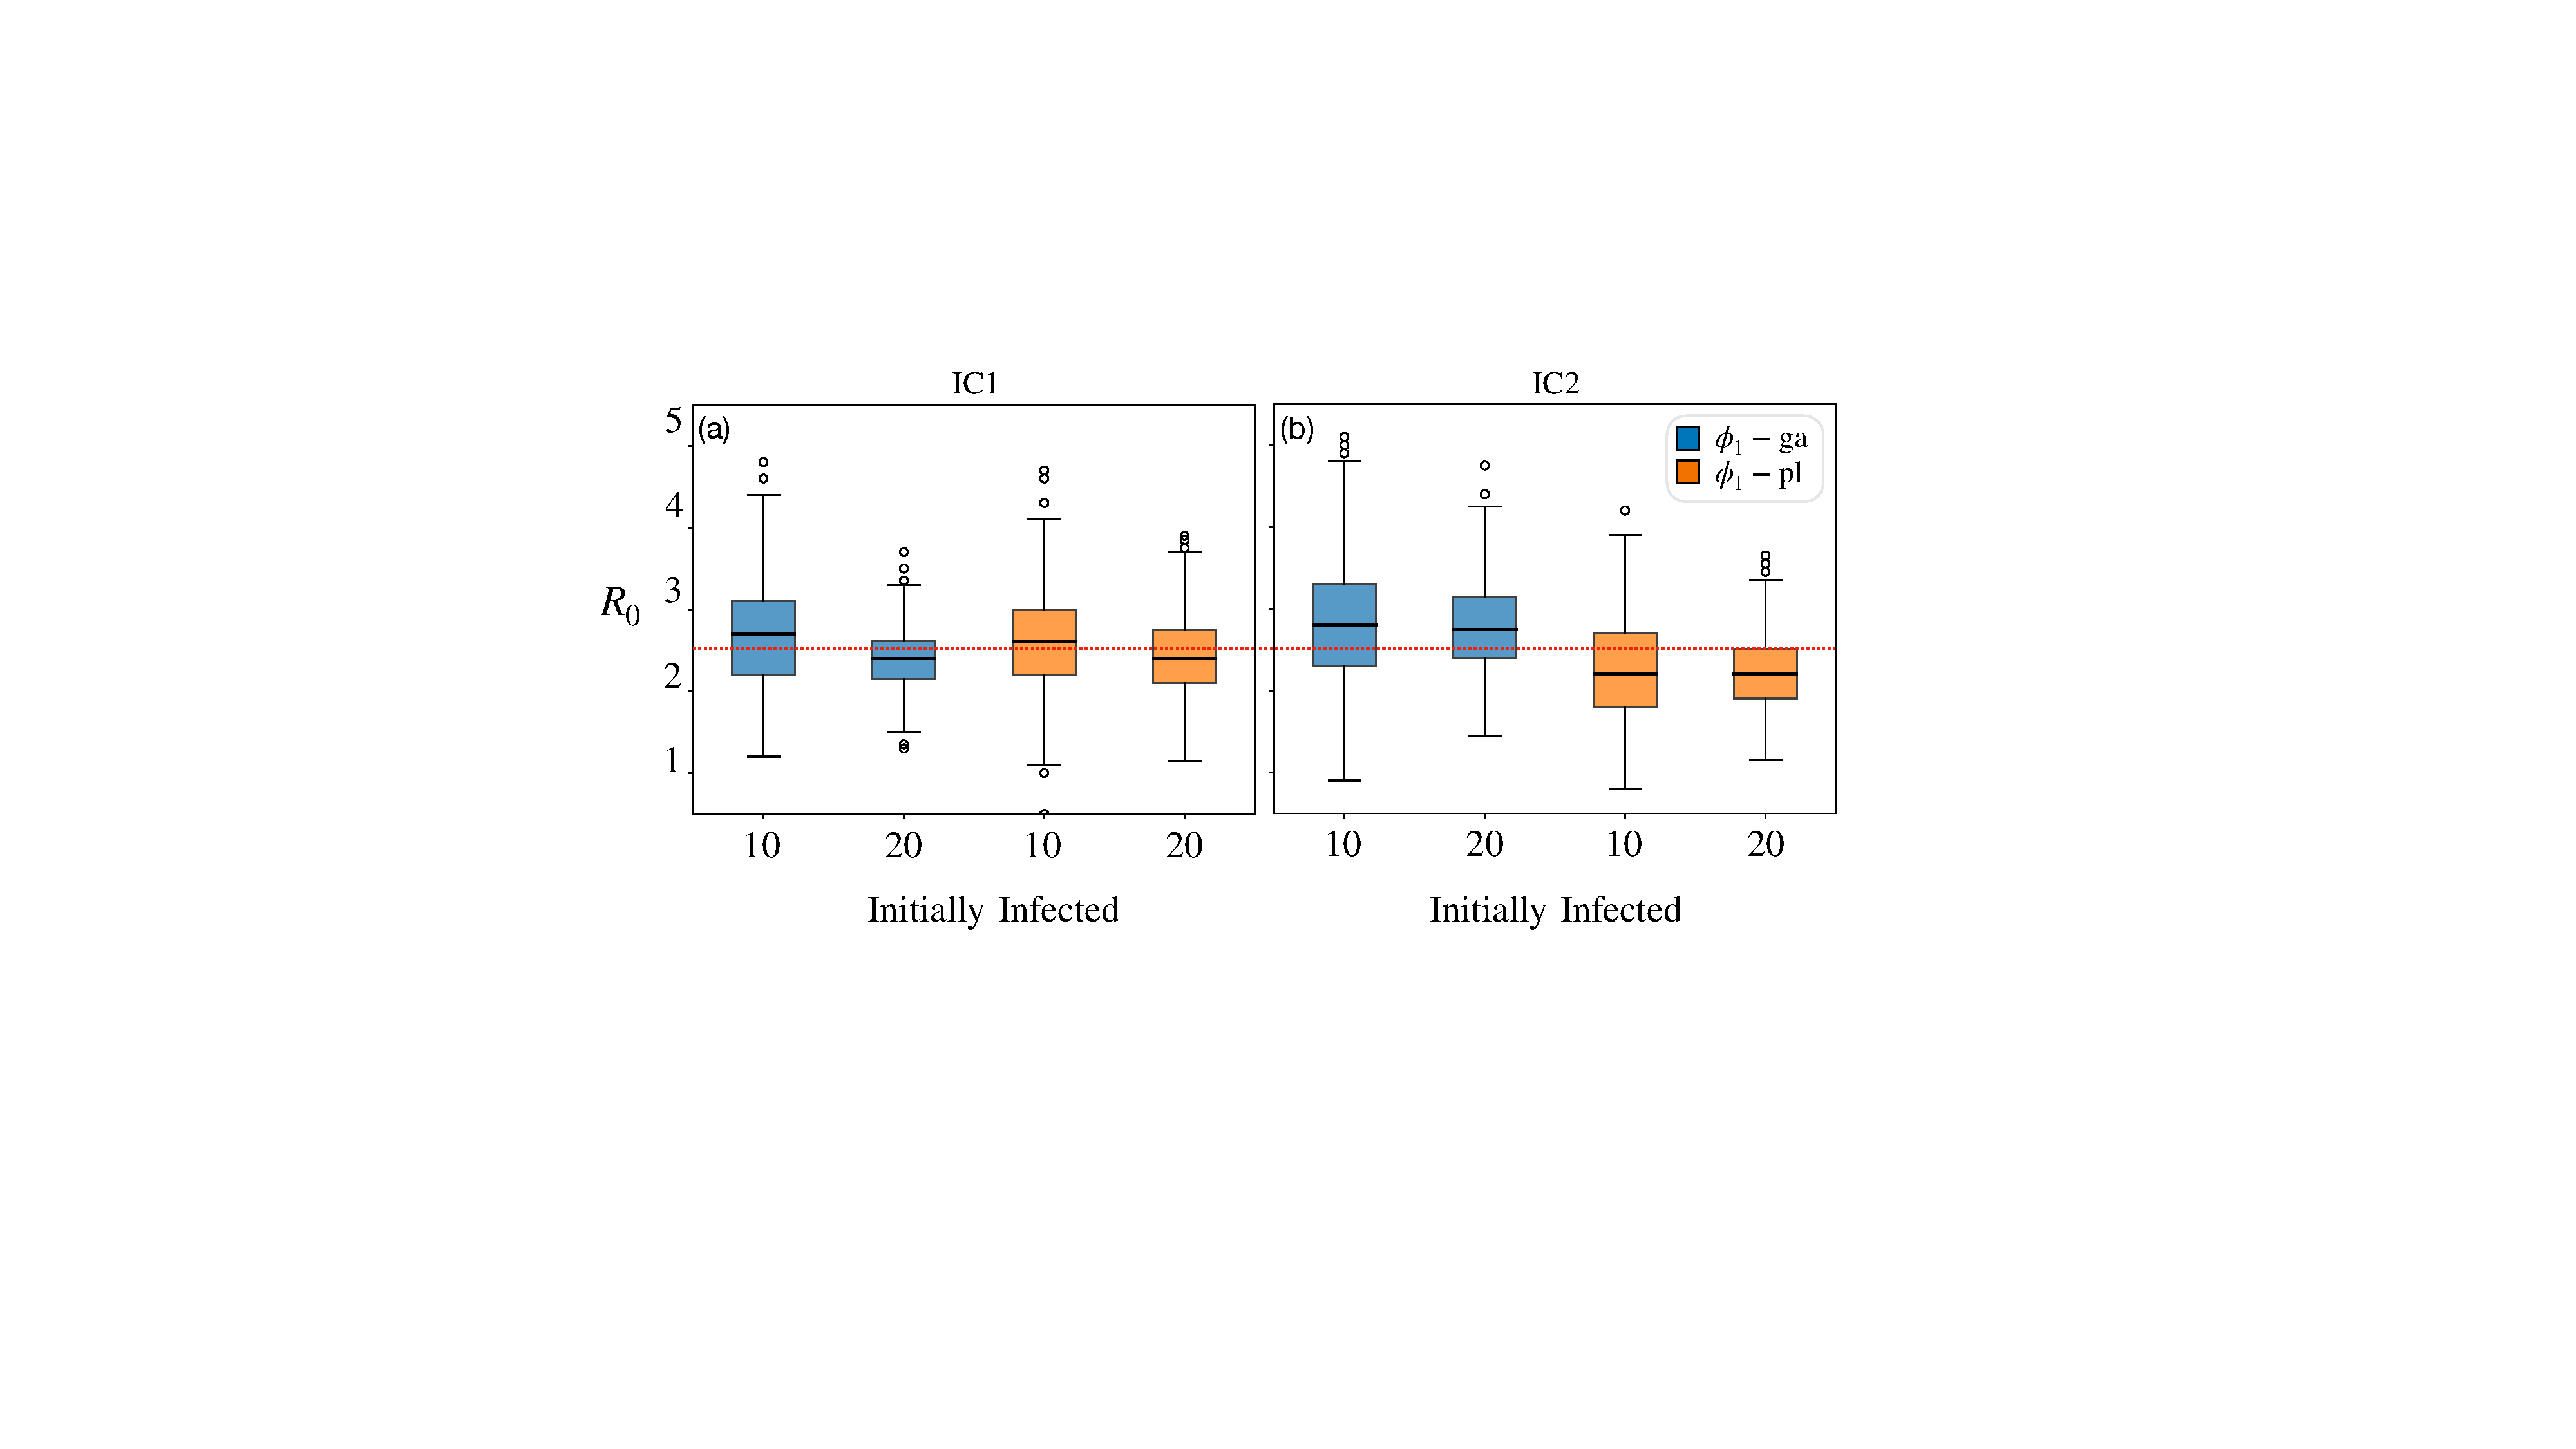
\includegraphics[scale=0.45]{chapter6/figures/fig5-IC.pdf}
    \caption{The value of $R_0$ is computed for 500 simulations with four different initial conditions at $t=0$ that varied A) the number of infected hosts at and B) the spatial locations of infected trees. 
    At time $t=0$, infected ash can be located either centrally (IC1), or scattered randomly (IC2) throughout the domain.
    The mean value of $R_0$ compares most similarly between models and number of infected ash when using IC1.
    Epidemic parameters for each ensemble: $\beta^*=1500$, $\rho_{avg}=0.017$, on a domain of size $\mathrm{2km\times 2km}$.}
    \label{fig:seir-ash-IC}
\end{figure}

In contrast, initial conditions had the opposite effect on inverse power law based epidemics.
For inverse power law spread, Figure \ref{fig:seir-ash-IC}(a-b) demonstrate that $R_0$ is generally lower for IC2 and higher for IC1.
Fat-tailed dispersal models thus demonstrate higher sensitivity to the domain boundary.
In particular, domain-sensitivity is demonstrated in \ref{fig:seir-ash-IC}(b), where more infected hosts are located closer to the domain edge.
These observations can be explained by realising that fat-tailed dispersal kernels are more likely to extend beyond the boundary.
Therefore, for the same normalised value of $\beta^*$, inverse power law models are more likely to undercount $R_0$ locally if measured inside a smaller domain.
Notwithstanding, secondary infections induced by $\phi_1$-pl spread over a wider area, and the effect of $R_0$-saturation is far less than $\phi_1$-ga.

Overall, $\overline{R}_0$ agreed closely between models when infected ash are placed at the domain centre IC1\textemdash indicated by distance of $\overline{R}_0$ about the red horizontal line.
Moreover, boundary effects and domain sensitivity was the least when using IC1.
Ensemble simulations of $R_0$ are thus chosen to evolve from the domain centre going forward.
Even though, for IC1, the epidemic impact is slightly lowered for Gaussian-based spread, on account of $R_0$-saturation; 
this points more towards a difference in model behaviour than artefacts of domain boundary size.


\subsection{Domain size $L$ and $R_0$}
\label{sec:r0-vs-L}

Before the small-scale $SEIR$ model of ADB can be spatially scaled up over GB, a suitable spatial and temporal scale must be chosen to measure $R_0$.
The purpose of this section is to compute $R_0$ over different sized domains from IC1, i.e. a small number of infected trees located at the domain centre at $t=0$.
Notably, it is desirable to choose a sufficient domain length, $L$, that accurately captures pathogen invasiveness within each model.
A suitable temporal scale of $R_0$-computations is set by the mean lifetime of infectious ash, five years.
Infected ash may survive for more extended periods, according to their exponentially distributed lifetimes, although this accounts for an increasingly small fraction of the host population.

Figures \ref{fig:ash-mortalty} and \ref{fig:seir-ash-IC} indicate that inverse power law dispersal exhibits a greater domain sensitivity than Gaussian kernels.
As remarked earlier, studies have shown that $R_0$ for crop disease can depend on the field size \cite{mikaberidze2016invasiveness} and saturates for a sufficiently large field.
Here, we have a similar scenario.
To capture $R_0$ in each $SEIR$ model, we require that $R_0$ should be computed inside a domain, such that it does not depend on the modelled area. 
Alternatively, repeated simulations inside a larger domain should produce the same $R_0$ value.
In contrast, running simulations inside a smaller domain will underestimate the reproductive ratio, and consequently, overall epidemic impact \cite{R0-perc-ref, time-varying-infectivity}.

Figure \ref{fig:r0-domain-size} reveals how both dispersal models relate to the domain-size.
By counting the number of secondary infections that result from the first-generation infected ash (at $t=0$), we may plot a distribution revealing how far away infections are likely to be produced.
Figures \ref{fig:r0-domain-size}(a-b) show the number of secondary infections induced a distance $D$ away from each infected source over $500$ repeated simulations.
Distributions for three different domain sizes are shown in Figure \ref{fig:r0-domain-size}(a-b).

Unsurprisingly, Figure \ref{fig:r0-domain-size}(a) and (b) reflect the Gaussian and inverse-power law dispersal kernels. 
However, Figure \ref{fig:r0-domain-size}(a-b) also show that secondary infections are unlikely to occur near first-generation infected ash.
A low secondary infection count close to infectious sources reflect the average space between hosts, set by $\rho$.
A higher density host distribution increases the relative proportion of induced secondary infections close to the source $<0.1\mathrm{km}$.

\begin{figure}
    \centering
    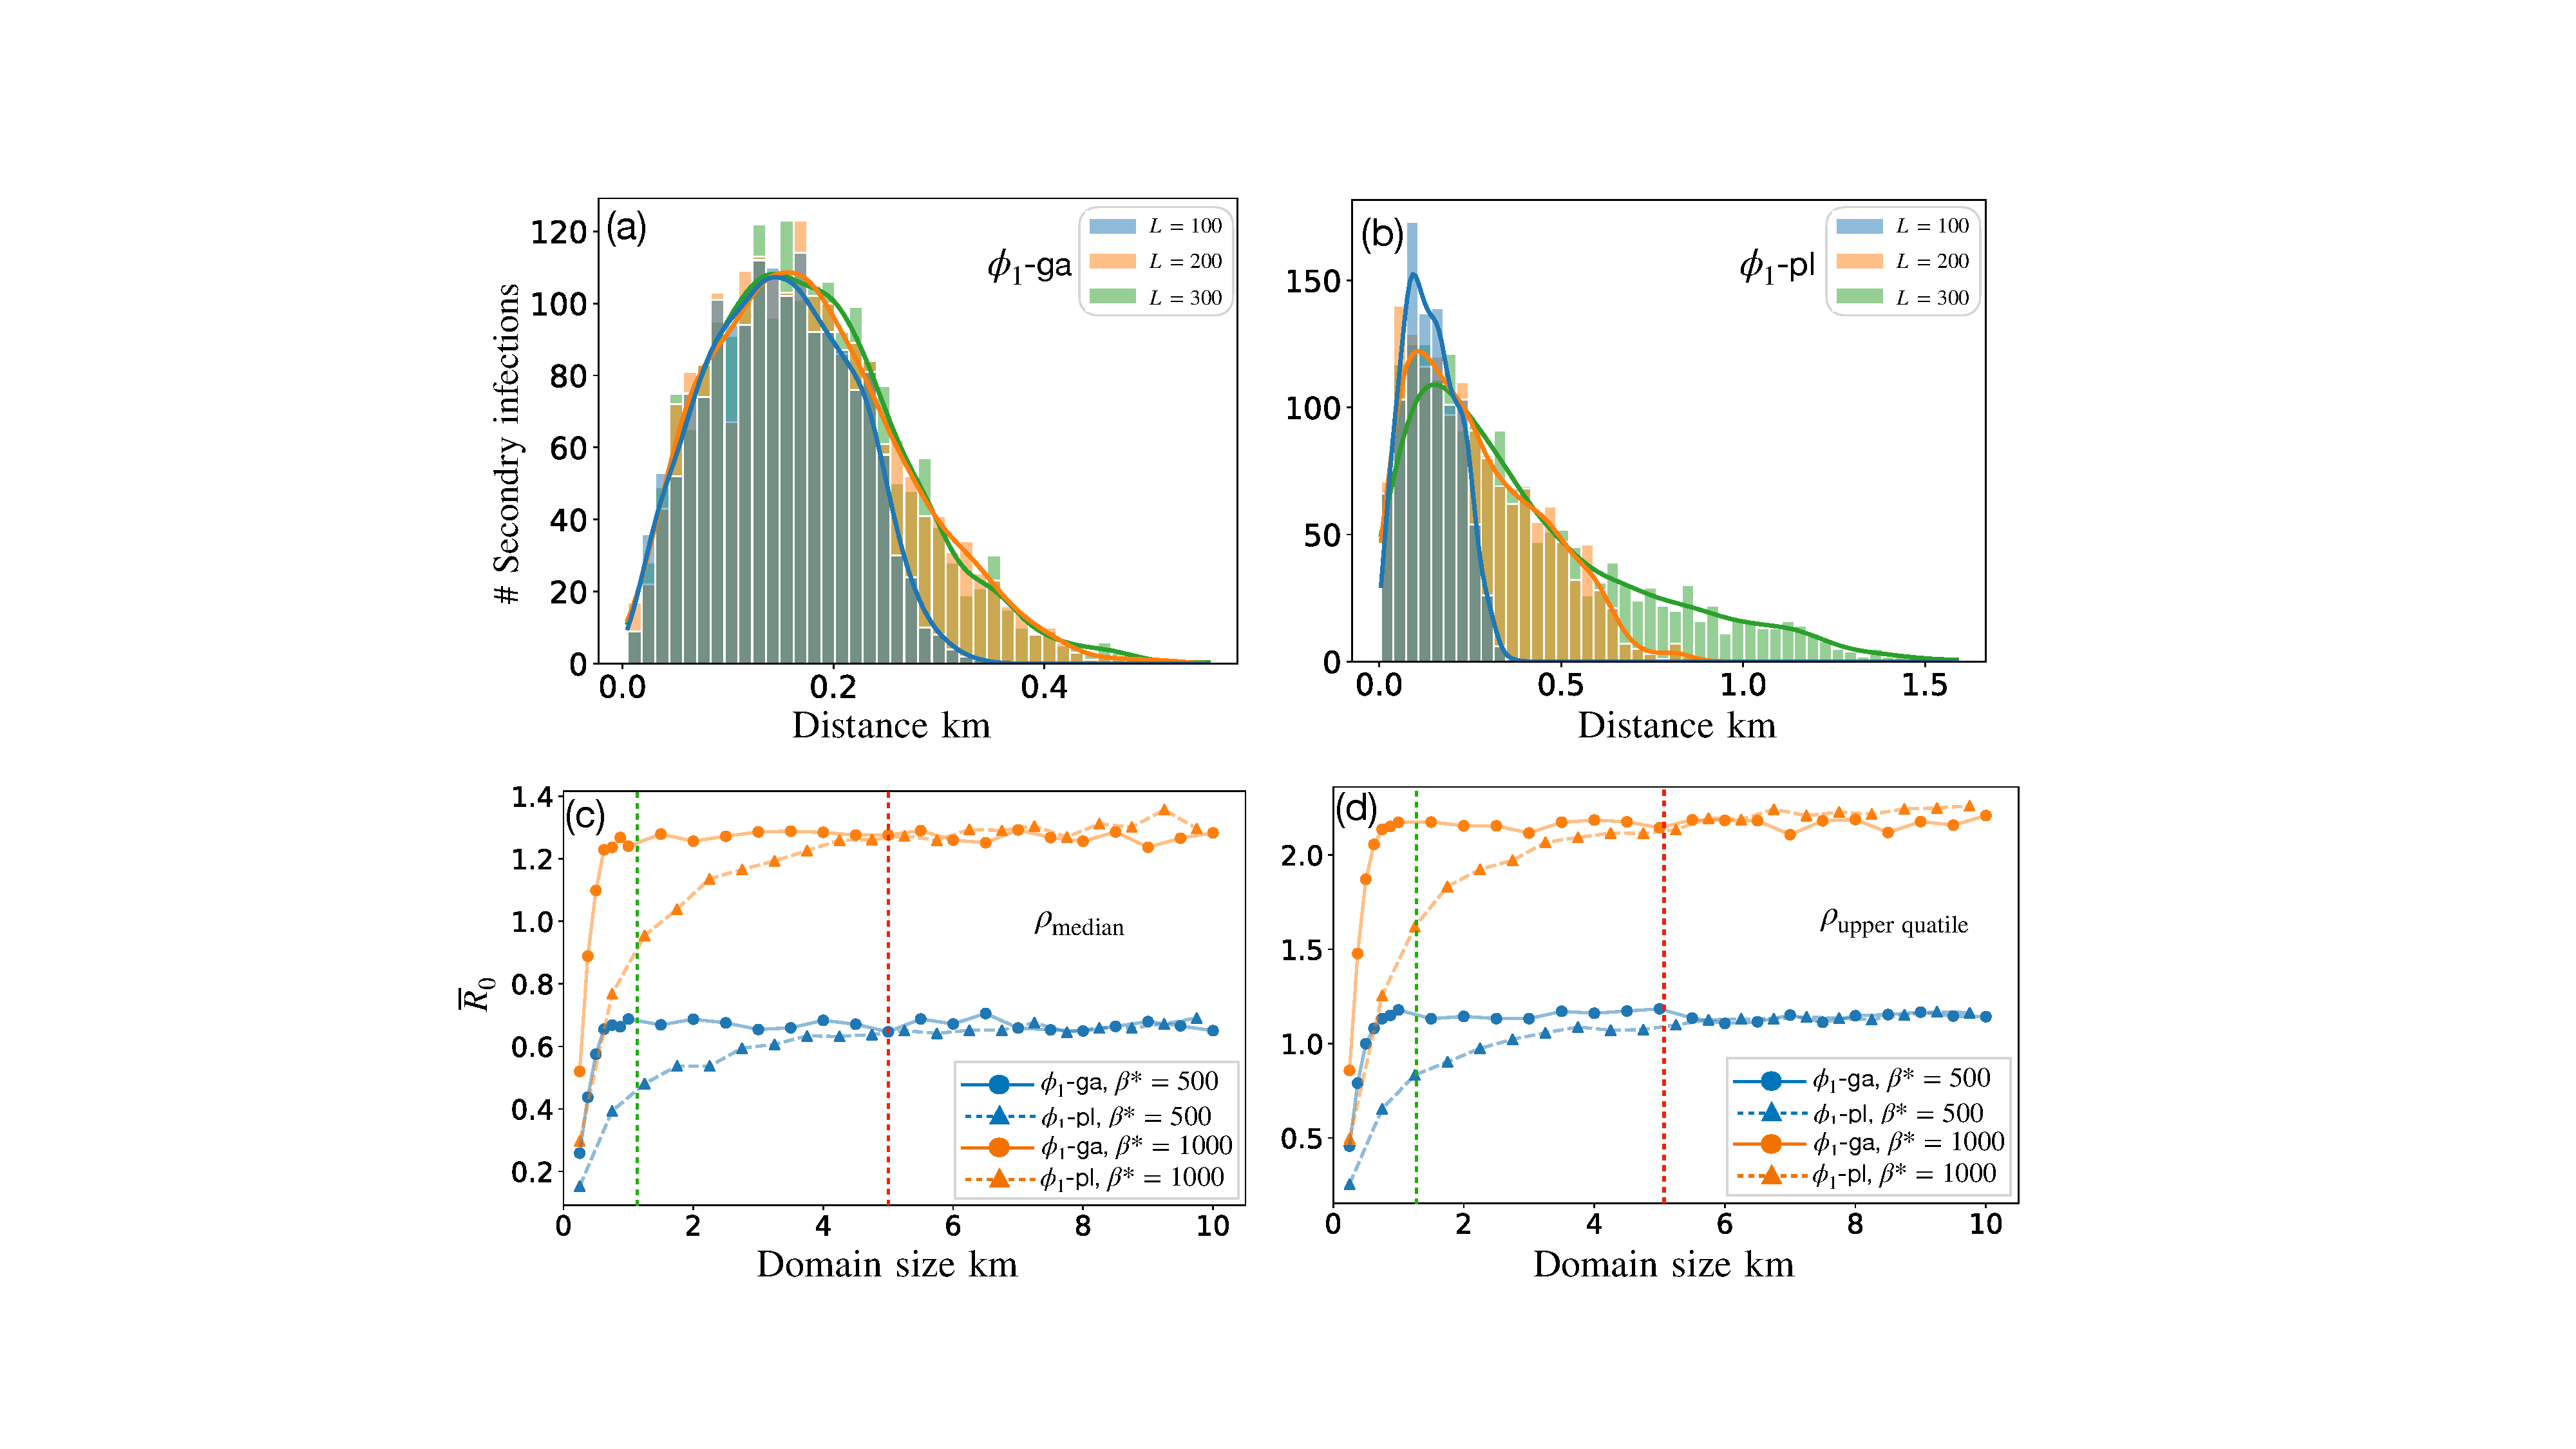
\includegraphics[scale=0.42]{chapter6/figures/fig5-R0-domain-size.pdf}
    \caption{The relationship between $R_0$ and the domain length, $L$. 
    For all panels, simulations run over five years or until the pathogen becomes extinct, whichever comes first.
    (a-b) Distributions show the number of secondary infections induced by distance over an ensemble of $500$ repeats for Gaussian and inverse power law dispersal kernels.
    Secondary infections are computed inside three different domain lengths of $L \in [100, 200, 300]$ (i.e. $\mathrm{500m\times500m,\ 1km\times1km,\ 1.5km\times1.5km}$) for epidemic parameters above threshold, $\beta^*=1000$ and $\rho_{avg} = 0.017$. Inverse power law spread demonstrates a higher domain sensitivity due to the fat-tailed kernel extending beyond the domain edge. (c-d) An ensemble-averaged reproductive ratio $\overline{R}_0$ is computed from $500$ repeated simulations over different domain lengths, up to a maximum of $L=2000$ or $\mathrm{10km \times 10km}$. The value of $\overline{R}_0$ is gauged at the median and upper quartiles of ash tree densities, (c) and (d), respectively, and at two infectivities shown in blue and orange. The value of $R_0$ saturates at around $\mathrm{1km\times1km}$ for Gaussian-based dispersal kernels and $\mathrm{5km\times5 km}$ for inverse power law dispersal kernels.}
    
    \label{fig:r0-domain-size}
\end{figure}

From Figure \ref{fig:r0-domain-size}(a-b) becomes visually apparent why domain sensitivity varies between dispersal models.
In Figure \ref{fig:r0-domain-size}(a), the number of infections is reduced for Gaussian dispersal at $L=100$, indicated by the smaller distribution tail in blue.
Although, increasing the domain length to $L=300$ produced no observable difference to $L=200$.
In all Gaussian simulations, no secondary infections were witnessed beyond $0.6\mathrm{km}$, in line with the results from \cite{grosdidier2018tracking}. 
On the other hand, a small number of secondary infections in the model $\phi_1$-pl can be seen up to the domain edge $1.5\mathrm{km}$ away.
Thus, if the domain size is below a minimum value of $L$, epidemics that observe inverse power law dispersal will be lowered due to an under-estimated total number of secondary infections.
For the exact value of $\beta^*$, $\phi_1$-pl can be seen to travel much further than $\phi_1$-ga and echos the difficulty of controlling fat-tailed pathogen dispersal \cite{WEBIDEMICS}, and more broadly, LDD.

Figures \ref{fig:r0-domain-size}(c-d) show how the mean value of $\overline{R}_0$ for each dispersal model saturates for a critical value of $L$, 
for two domains at the median and upper quartile of ash density $\rho_{med}=0.011$ and $\rho_{uq}=0.019$ (a) and (b) respectively.
Simulations for two infectivity parameters $\beta^* \in [500, 1000]$ are shown in blue and orange.
The computed value of $\overline{R}_0$ shows the aforementioned characteristic increase, up to a maximum saturation value.
Each infectivity and tree density combination produced a similar saturation point of $L \approx 1\mathrm{km}$ for $\phi_1$-ga and $L\approx 5\mathrm{km}$ for $\phi_1$-pl, the vertical green and red lines, respectively. 

From Figures \ref{fig:r0-domain-size}(c-d), a suitable domain length $L$ can be ascertained for each dispersal model, 
found to be $\mathrm{1km\times1km}$ for models $\phi_1$-ga and $\phi_2$-ga, and $\mathrm{5km\times5km}$ for models $\phi_1$-pl and $\phi_2$-pl. 
Moving onward, a proper characterisation of the GB ash tree canopy cover data set produced by \cite{hill.data} will be conducted,
before we determine $R_0$ as a function of host density in section \ref{section:r0-tree-density}.

\section{Constructing $R_0$-maps over Great Britain}

\label{sec:r0-map-construct}
In this section, $R_0$ values of the small-scale $SEIR$ model of ADB will be projected onto the host distribution of ash, 
given by \cite{hill.data}, to create landscape-level $R_0$-maps over Great Britain. 
Doing so will permit the investigation of a novel control strategy in chapter \ref{ch7:landscape-level-control} 
and allow the local-scale epidemic severity, based on tree-to-tree interactions, to be efficiently scaled over large areas.

\subsection{Ash host distribution}

\begin{figure}
    \centering
    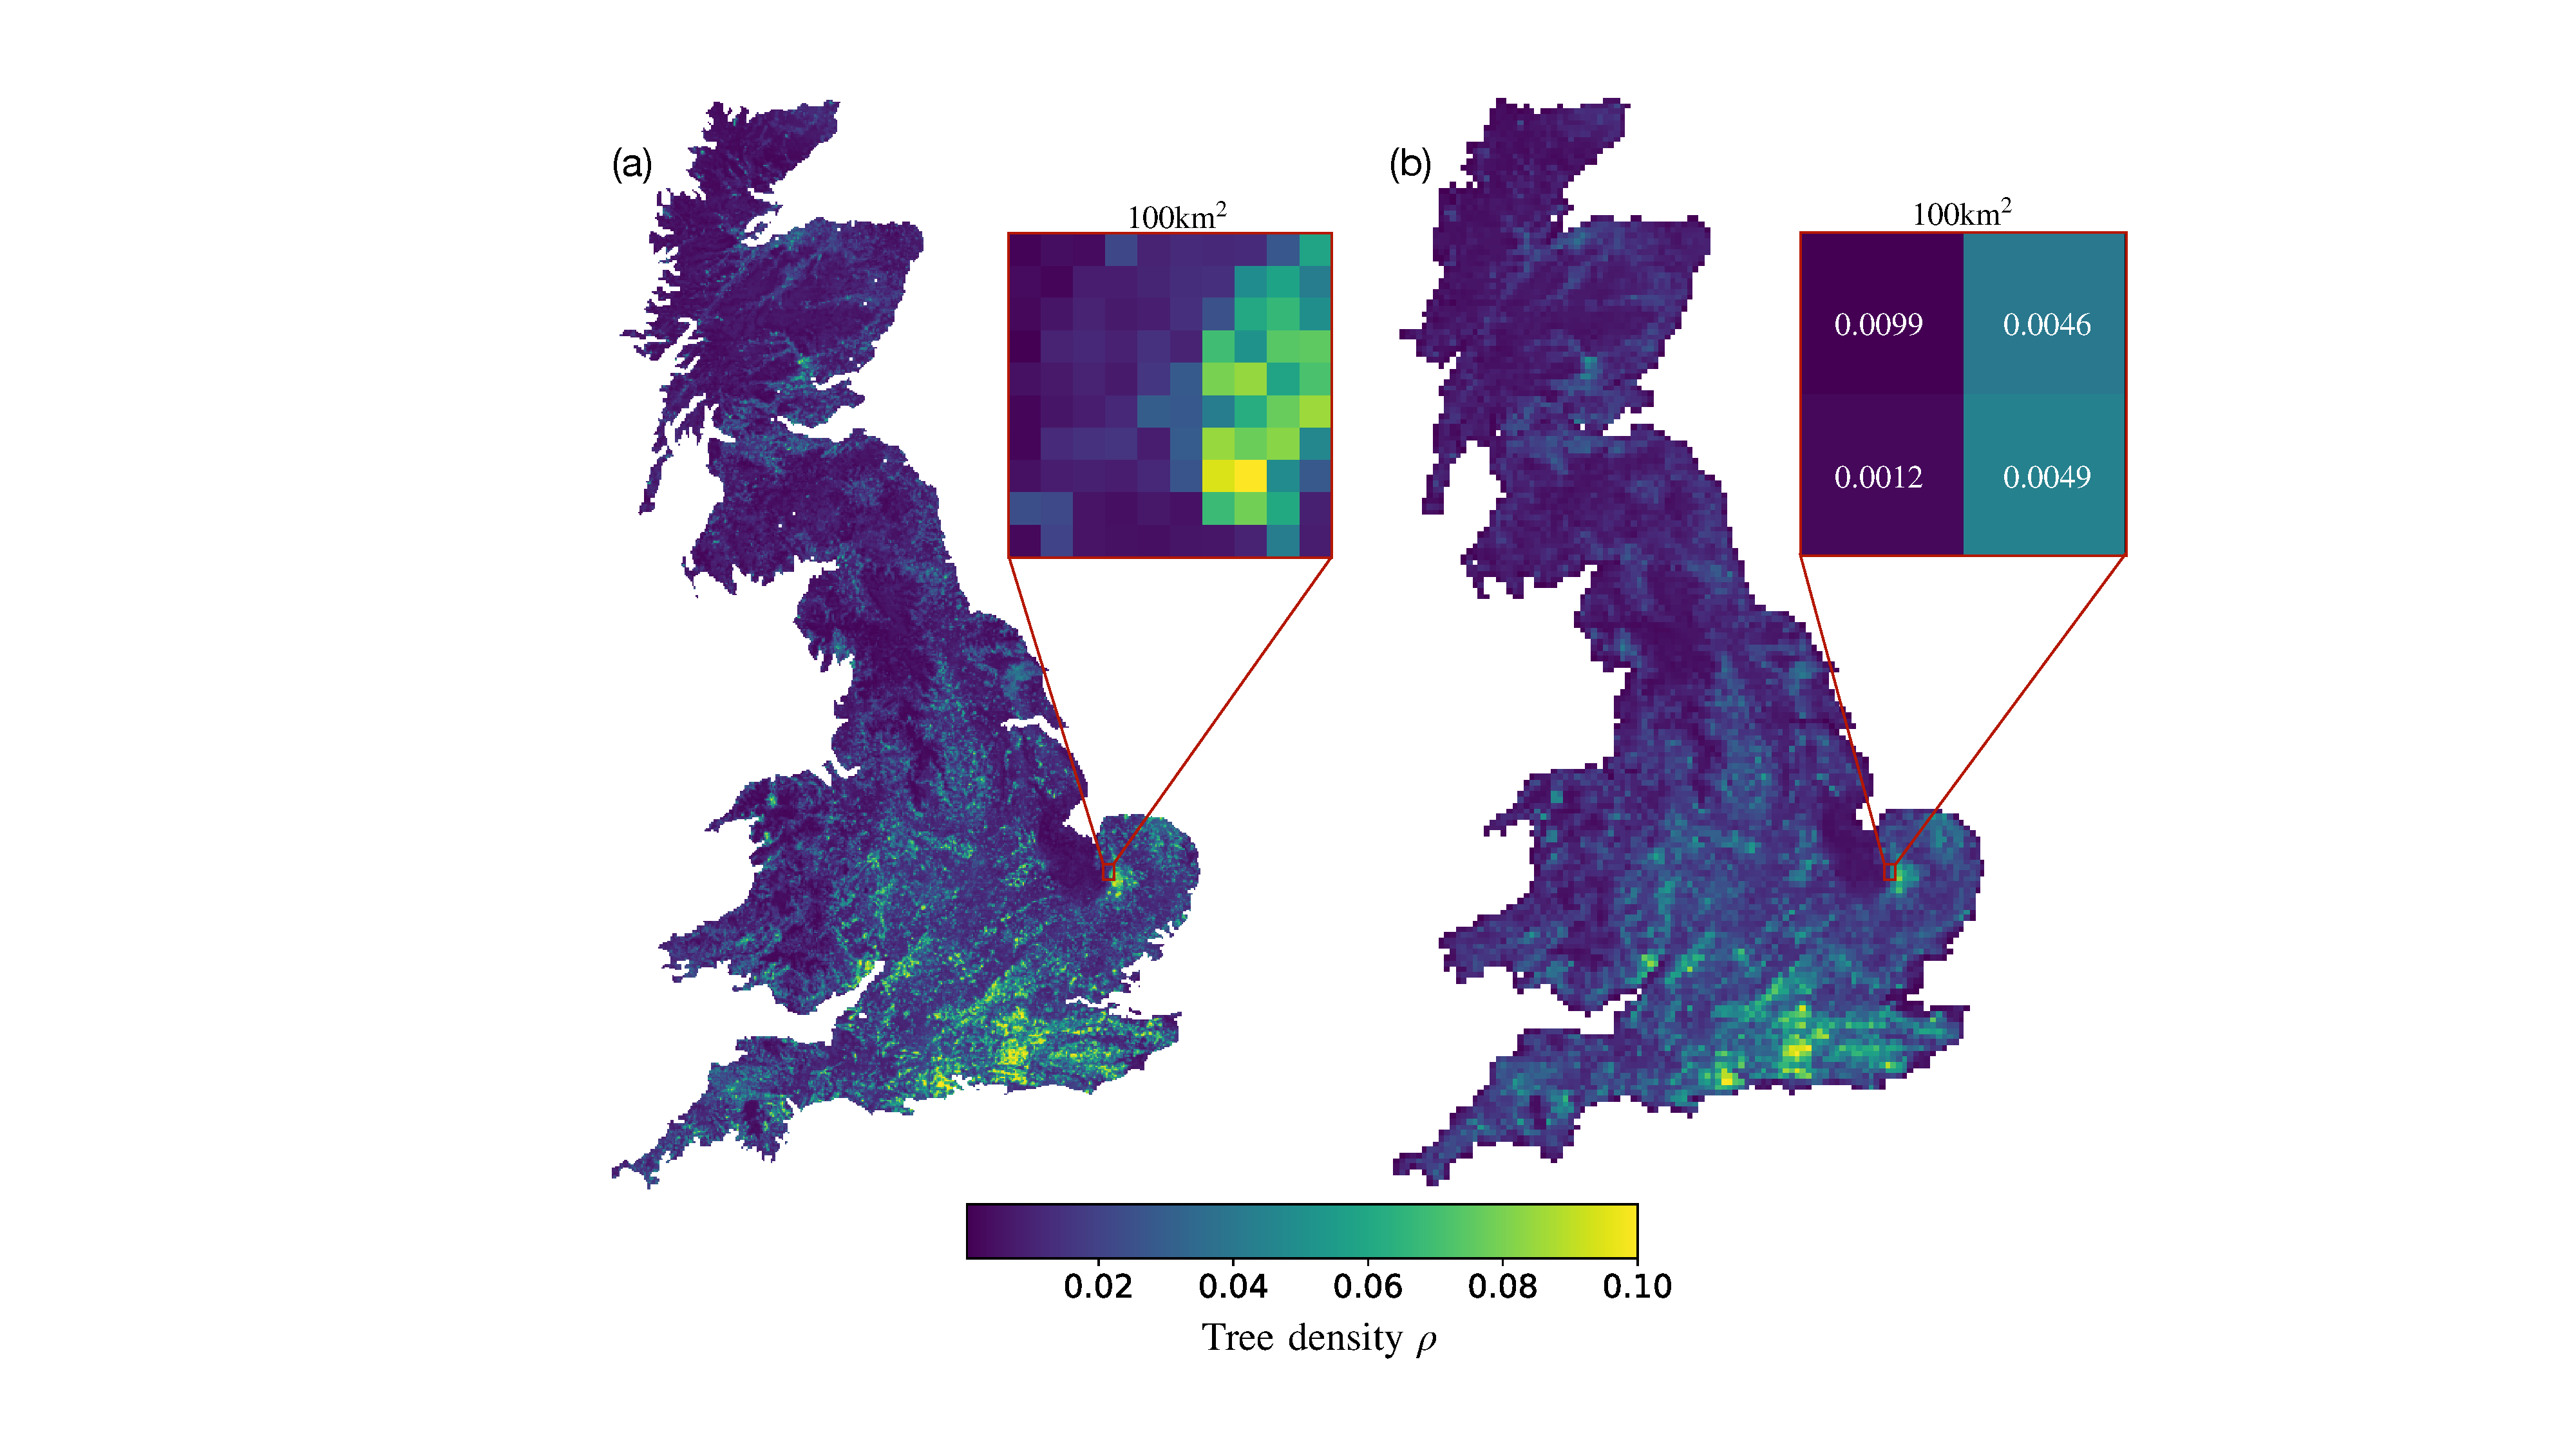
\includegraphics[scale=0.45]{chapter6/figures/fig-ash-data.pdf}
    \caption{The ash canopy cover data, as modelled by \cite{hill.data}, is converted into a map of tree density. (a) A map of ash densities at the original resolution of $1\mathrm{km} \times 1\mathrm{km}$, the inset consisting of $10\times 10$ pixels (b) A coarse-grained map of ash densities at a resolution of $5\mathrm{km} \times 5\mathrm{km}$, the inset consists of $2 \times 2$ pixels. Both insets show the same $100\mathrm{km^2}$ area, and illustrates how coarse-graining the host distribution results in a loss of spatial structure. A small number of densities over $10\%$ were excluded from the density-map.}
    \label{fig:ash-host-data}
\end{figure}

Ash densities are parameterised by modelled ash abundance data provided by \cite{hill.data}. 
Previously, the oak canopy cover dataset given by \cite{hill.data} was used previously in chapter \ref{fig:ch4_uk_spread} alongside a toy model of landscape-level tree disease.
The canopy cover datasets produced by \cite{hill.data} combine several data sources that partly cover Great Britain, 
regression methods then extrapolate canopy cover over the whole of Great Britain.
Conveniently for the present chapter, ash happened to be among the most accurate data sets given by \cite{hill.data}. 
For a more in-depth description of the methods used by \cite{hill.data} and a review of host data in general, see chapter \ref{chapter:lit-rev}.

Modifications had to be made to the modelled ash canopy cover data to complement the $SEIR$ model. 
Firstly, the raw abundance values were re-scaled into a dimensionless tree density $\rho$. 
The exact process was outlined in chapter \ref{ch5:dispersal-model} 
i.e. by converting the units $\mathrm{ha/km^2}$ to kilometre-squared of ash cover per kilometre-squared of land. Secondly, 
the domain resolution has to be re-scaled to reflect the spatial scale of local wind-borne dispersal, as parameterised by \cite{grosdidier2018tracking}.
Lastly, the small number of patches with exceedingly high densities were capped to $\rho_{max} = 0.10$, thus forming a hard upper limit in the density map.

Figure \ref{fig:ash-host-data}(a) shows a density map of ash, at the original resolution of $\mathrm{1km}\times \mathrm{1km}$, produced from abundance data given by \cite{hill.data}.
The inset shows a block of $10\times10$ pixels, each of size $1\mathrm{km} \times 1 \mathrm{km}$.
In the small-scale Gaussian dispersal-based $SEIR$ model, a domain size of $\mathrm{1km}\times \mathrm{1km}$ was shown sufficient to measure the average $R_0$ over a five-year period \textemdash demonstrated by Figures \ref{fig:r0-domain-size}(c-d).
However, the inverse power law models required a larger domain size of $\mathrm{5km}\times \mathrm{5km}$ to prevent underestimating epidemic severity.
Figure \ref{fig:ash-host-data}(b) shows the host distribution coarse-grained to a resolution of $\mathrm{5km}\times \mathrm{5km}$ pixels.
The insets of Figures \ref{fig:ash-host-data}(a-b) compare the same region.
Although, in Figure \ref{fig:ash-host-data}(b), pixels are effectively averaged representing larger $5\mathrm{km} \times 5 \mathrm{km}$ patches.
The resulting domain is smoother and therefore losses spatial structure.

From Figures \ref{fig:ash-host-data}(a-b), the south of England contains the highest concentration of high-density ash patches, and ash become progressively less abundant in Scotland and coastal locations, 
in western Wales, for example. 
A higher density of ash can be expected to yield a higher number of secondary infections, in line with the results of chapters \ref{ch3:two-param-model} and \ref{ch5:dispersal-model}.

\subsection{Tree density and $R_0$}
\label{section:r0-tree-density}

Figures \ref{fig:R0-map-generation}(a-c) illustrated the relationship between $R_0$ and ash density.
Figure \ref{fig:R0-map-generation}(a) shows a PDF (probability density function) of ash densities $\rho$ over the map of Great Britain\textemdash overlaid with a KDE shown in red.
As noted above, few locations support densities of $\rho=0.10$ and over\footnote{
The original $\mathrm{1km \times 1km}$ map resolution contained $2.2\times 10^4$ $1\mathrm{km^2}$ data points, 
with some outlier pixels having densities in the interval $\rho \in [0.10, 0.30]$ which were excluded from the analysis due to 
A) the increased computational run-time required to simulate the $SEIR$ model of ADB  
B) densities beyond $0.10$ account for a negligible portion of the overall population.}. 
Between the limits of $\rho \in [10^{-2}, 10^{-1}]$, the PDF follows a power law of the form $\sim \rho ^{-k}$, as evident from linearity in the logarithmic inset axes.
The distribution had a fitted exponent of $k=1.90$, shown by the black line; 
intriguingly, this observation suggests self-similarity in the data.

Figures \ref{fig:R0-map-generation}(b-c) contrast the behaviour between $R_0$ and tree density $\rho$ for linear and peaked sporulation functions, $\phi_1$ and $\phi_2$ respectively.
Values of $R_0$ were ensemble-averaged over $100$ repeated simulations.
For the two values of infectivity, $\beta^*\in [500, 1000]$ shown, all model variants display the same linearity between $R_0$ and $\rho$ \textemdash also explored in chapter \ref{ch5:dispersal-model}.
The dashed orange and blue lines show how high values of $\beta$ and $\rho$ result in a considerable value of $R_0$.
For high $R_0$ values, the Gaussian dispersal models $\phi_1$-ga and $\phi_2$-ga begin to deviate from linearity as density is increased,
due to the phenomena of $R_0$-saturation witnessed in section \ref{section:initial-conditions}.
Figure \ref{fig:R0-map-generation}(b) reveals a larger area of shaded grey, 
suggesting that the sole difference between sporulation models is that $\phi_2$-ga deviates from linearity more than $\phi_1$-ga.

In Figures \ref{fig:R0-map-generation}(b-c), the regime of pathogen extinction is indicated by the horizontal red lines, 
which correspond to a critical `density threshold' denoted by $\rho_c$ (equivalent to the threshold $R_0 = 1$).
When used in conjunction with the data-set from \cite{hill.data}, Figures \ref{fig:R0-map-generation}(b-c) represent an appropriate projection of $R_0$ over the map of Great Britain.
Below the threshold $R_0=1$, infected ash can still survive and reproduce (i.e. persist below the threshold, as we saw in Figure \ref{fig:SEIR-spread}(c)), albeit at slower rates.
Negating below-threshold patches is a vital assumption\textemdash discussed more below.

\begin{landscape}
\begin{figure}
    \centering
    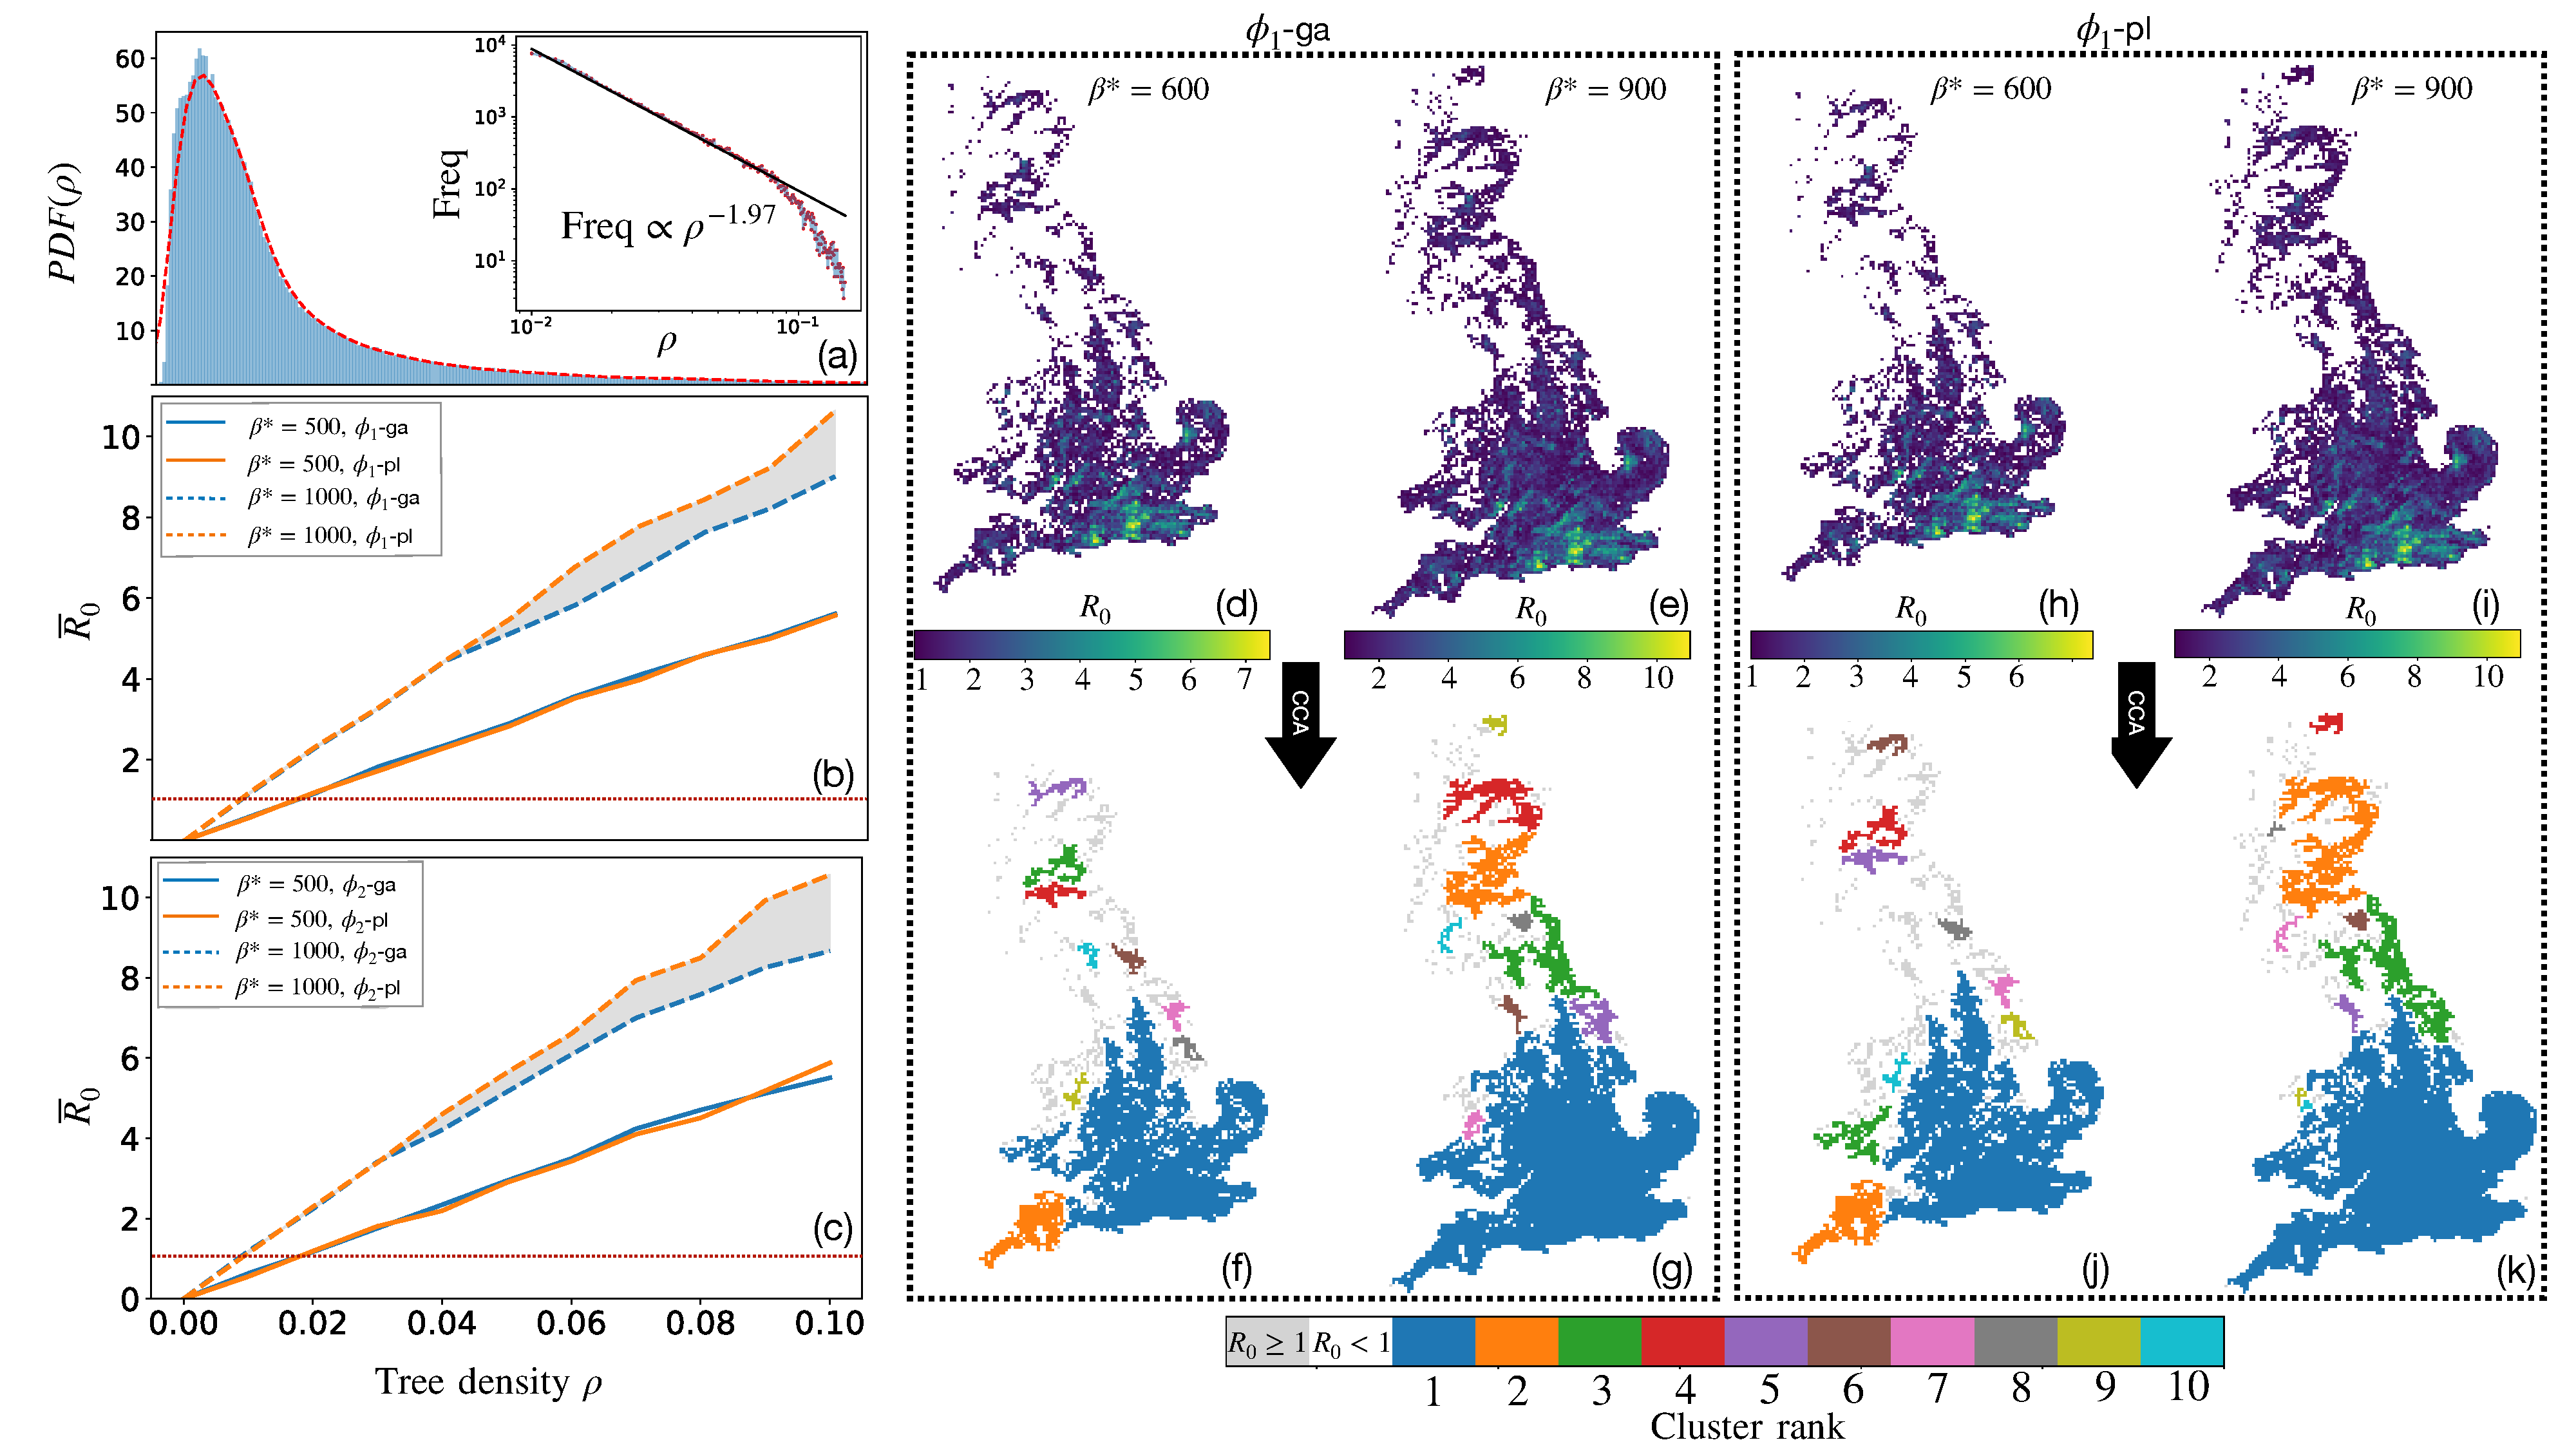
\includegraphics[scale=0.38]{chapter6/figures/fig6-R0-map-generation.pdf}
    \caption{Generating $R_0$ maps for ADB over Great Britain. (a) Ensemble-averaged results of $R_0$ are plotted against the tree densities informed by \cite{hill.data}, revealing a linear relation between $R_0$ and $\rho$. (b-c) Projecting $SEIR$ inverse power law $R_0$ values onto the re-scaled $5\mathrm{km} \times 5 \mathrm{km}$ ash host-distribution for two values of $\beta_{pl}$. Patches of land below $R_0 = 1$ are shown as white space. (d-e) The top $10$ largest connected, and susceptible, $R_0$-clusters that are present in maps (b-c).}
    \label{fig:R0-map-generation}
\end{figure}
\end{landscape}

Figures \ref{fig:R0-map-generation}(d-e) and (h-i) present $R_0$-values of the small-scale $\phi_1$-ga and $\phi_1$-pl $SEIR$ models projected onto the host distribution of ash.
Both sets of $R_0$-maps are projected onto the same coarse-grained $5\mathrm{km} \times 5\mathrm{km}$ re-scaled host distribution.
For all variants of the $SEIR$ model, $R_0$-maps compared similarly\textemdash shown for the two values of infectivity, $\beta^* \in [600, 900]$.
All locations below the transmission threshold $R_0=1$ were given numerical values of zero and are depicted by inland white space.
Under the influence of a more infectious pathogen, larger areas of the ash population become susceptible by supporting the growth and reproduction of the pathogen, illustrated by the difference in patch density in Figures \ref{fig:R0-map-generation}(b-c). 
Importantly, each $R_0$-valued pixel portrays the local-scale epidemic impact experienced at that location, predicted from a five-year ensemble-averaged value of $R_0$.

Suppose that a fitted value of infectivity $\beta^*$ is found to fall within a standard error of $SE=250$,  i.e. $\beta^* = 750 \pm 250$.
In this scenario, epidemic uncertainty is captured by the divergence between dashed and solid lines in Figures \ref{fig:R0-map-generation}(b-c)
and conveniently visualised by differences in the resulting $R_0$-maps.
Although landscape-level heterogeneity and regional susceptibility can be loosely identified from $R_0$-maps in Figures \ref{fig:R0-map-generation}(d-i),
visualising differences between model variants is untenable due to their similarity. 
Furthermore, determining which pixels connect to form susceptible clusters is non-trivial. 
To this aim, the next section will present a means to identify clustering in $R_0$-maps.

\subsection{Clustering in the $R_0$ map}
\label{sec:r0-clustering}

An image processing technique called `connected component analysis' (CCA) was used to identify and label susceptible clusters and simplify the $R_0$-map \cite{CCA1, CCA2} . 
The Python-SciPy package `ndimage' \cite{scipy} was used to implement CCA via the function `label'. 
Doing so labelled all susceptible neighbours as connected members of the same cluster, according to a structuring element \cite{liang1989erosion}. 
That is, if two susceptible patches of ash lie within the same neighbourhood, defined by the structuring element, they are connected members of the same cluster\footnote{Structuring elements have their roots in shape, and image analysis \cite{23111}, where they define how distinct binary shapes connect to form images \cite{liang1989erosion, nachtegael2001connections}}. 
More information on structuring elements and CCA can be found in \textcolor{red}{Appendix \ref{a:R0-map-construction}}. % To fill in Appendix

Moore and Von-Neumann neighbourhoods were chosen as structuring elements to classify connected components\textemdash a comparative look exploring the differences between Von-Neumann and Moore 
structuring elements is resumed below in sections \ref{sec:inverse-power-law-r0-clustering}-\ref{sec:ga-r0-clustering}.  
Figures \ref{fig:R0-map-generation}(f-k) correspond to the top ten largest connected $R_0$-clusters (by area $\mathrm{km^2}$) present in the $R_0$-maps of Figures \ref{fig:R0-map-generation}(d-i) according to the Moore neighbourhood.
For both dispersal models, increasing the infectivity parameter $\beta$ leads to a more susceptible and connected $R_0$-map, as demonstrated by the larger dominating cluster in Figures \ref{fig:R0-map-generation}(g) and (k).

There are little to no differences between how Gaussian and inverse power law models spatially scale, according to the raw $R_0$-maps of Figures \ref{fig:R0-map-generation}(d-i).
However, CCA reveals some subtle differences in the projection of $\phi_1$-ga and $\phi_1$-pl under the same normalised infectivity parameter $\beta^*$.
Although, given similar gradients in the graph of $R_0$ versus $\rho$ for lower infectivity values
\textemdash demonstrated by the convergence of solid orange and blue lines in Figures \ref{fig:R0-map-generation}(b-c)\textemdash 
Gaussian and inverse power law models should produce the exact $R_0$-map.
In contrast, for higher infectivity parameters, we might expect the inverse power law model to yield a more susceptible map, as per Figures \ref{fig:R0-map-generation}(b-c) when the Gaussian model deviate below linearity.

For the infectivity parameter $\beta^*=600$, model $\phi_1$-ga shows that the largest `dominating' cluster (in blue) extends over a slightly larger area than for model $\phi_2$-pl.
In Figure \ref{fig:R0-map-generation}(j), the third-largest cluster (in green, located in Wales) remains disconnected from the largest dominating cluster (shown in blue),
whereas in Figure \ref{fig:R0-map-generation}(f) the corresponding clusters are connected. 
In a similar vein, Figure \ref{fig:R0-map-generation}(k) shows a larger dominating cluster than Figure \ref{fig:R0-map-generation}(g).
However, differences are seen most visibly over Scotland and Northern England (Humber-Northumbria), where the second and third largest-ranked clusters extend over more significant areas.
Nevertheless, differences in how dispersal models scale over GB are primarily trivial, and stochasticity in ensemble-averaged $R_0$-values could likely explain any differences.

\subsection{Interpreting susceptible $R_0$-clusters}

Given that disease gradients can extend over $10-1000\mathrm{km}$, we cannot preclude the possibility of secondary infections spreading between clusters.
Alongside jumping directly over below-threshold patches, the pathogen may use intermediary trees inside below-threshold patches as stepping stones and jump between clusters indirectly. 
Conceptually, this has been described for pathogens jumping between crop fields \cite{Gilligan-disease-management} and more abstract modelling work \cite{wingen2013long}.
In a simplified interpretation, the model presents two distinct types of spread, within-cluster and between-cluster spread. 

Here, within-cluster connectivity is sufficient for uninhibited spore-dispersal between nearest-neighbour patches in the $SEIR$ model of ADB.
Moreover, the disease may spread over large spatial scales even without the need for LDD\textemdash without directly or indirectly, jump between nearest-neighbours.
Thus, high-risk areas can be simplistically identified in the $R_0$-map.
Next, a closer look at $R_0$-clustering is conducted.

\subsection{Inverse power law $R_0$-map clustering}
\label{sec:inverse-power-law-r0-clustering}
% explain basic behaviour, 5km spatial structure

In the small-scale $SEIR$-model of ADB, inverse power law dispersal required a domain size of $\mathrm{5km \times 5km}$ to accurately gauge $R_0$ over the mean infectious lifetime of ADB.
Domain size, $L$, in the inverse power law $SEIR$ models, therefore, motivate a coarse-grained host distribution.
Consequently, when spatially scaling the inverse power law model over Great Britain, each pixel reflects a $\mathrm{5km \times 5km}$ patch of land at minimum.
It would be possible to possible to coarse-grain to lower resolutions, e.g. $\mathrm{10km \times 10km}$.
Although as Figure \ref{fig:ash-host-data}(b) eludes to, landscape-level spatial structure is lost in the process.
Therefore, the inverse power law models $\phi_1$-pl and $\phi_2$-pl were explored over a single landscape-level resolution of $\mathrm{5km \times 5km}$.

For each value of infectivity, an $R_0$-map will contain a variety of differently sized $R_0$-clusters.
Figure \ref{fig:inverse-power-law-clustering} presents $R_0$-clustering behaviour for the inverse power law model.
A proper understanding of clustering can be achieved by exploring how the distribution of cluster sizes change in response to infectivity. 
Figures \ref{fig:inverse-power-law-clustering}(a) and (c) show the frequency distribution of cluster sizes, 
for models $\phi_1$-pl and $\phi_2$-pl respectively.
The distributions depict cluster sizes for three infectivity parameters $\beta^* \in [250, 500, 1000]$ according to the Moore neighbourhood.
In both frequency distributions, a small proportion of large dominating clusters can be seen alongside more numerous smaller $R_0$-clusters.

Unsurprisingly, a lower infectivity parameter reduces the size of the highest-ranked cluster and lowers the overall coverage of susceptible $R_0$-clusters\textemdash shown in blue.
Increasing the infectivity produces a larger dominating cluster but reduces the mean size of lower-ranked $R_0$-clusters, 
understood by contrasting the orange and green frequency distributions.
The inset plots of Figure \ref{fig:inverse-power-law-clustering}(a) and (c) depict the same behaviour in a rank-ordered list of the top 25 largest $R_0$-clusters by size.
Both sporulation models display the same fundamental relationship.

\begin{figure}
    \centering
    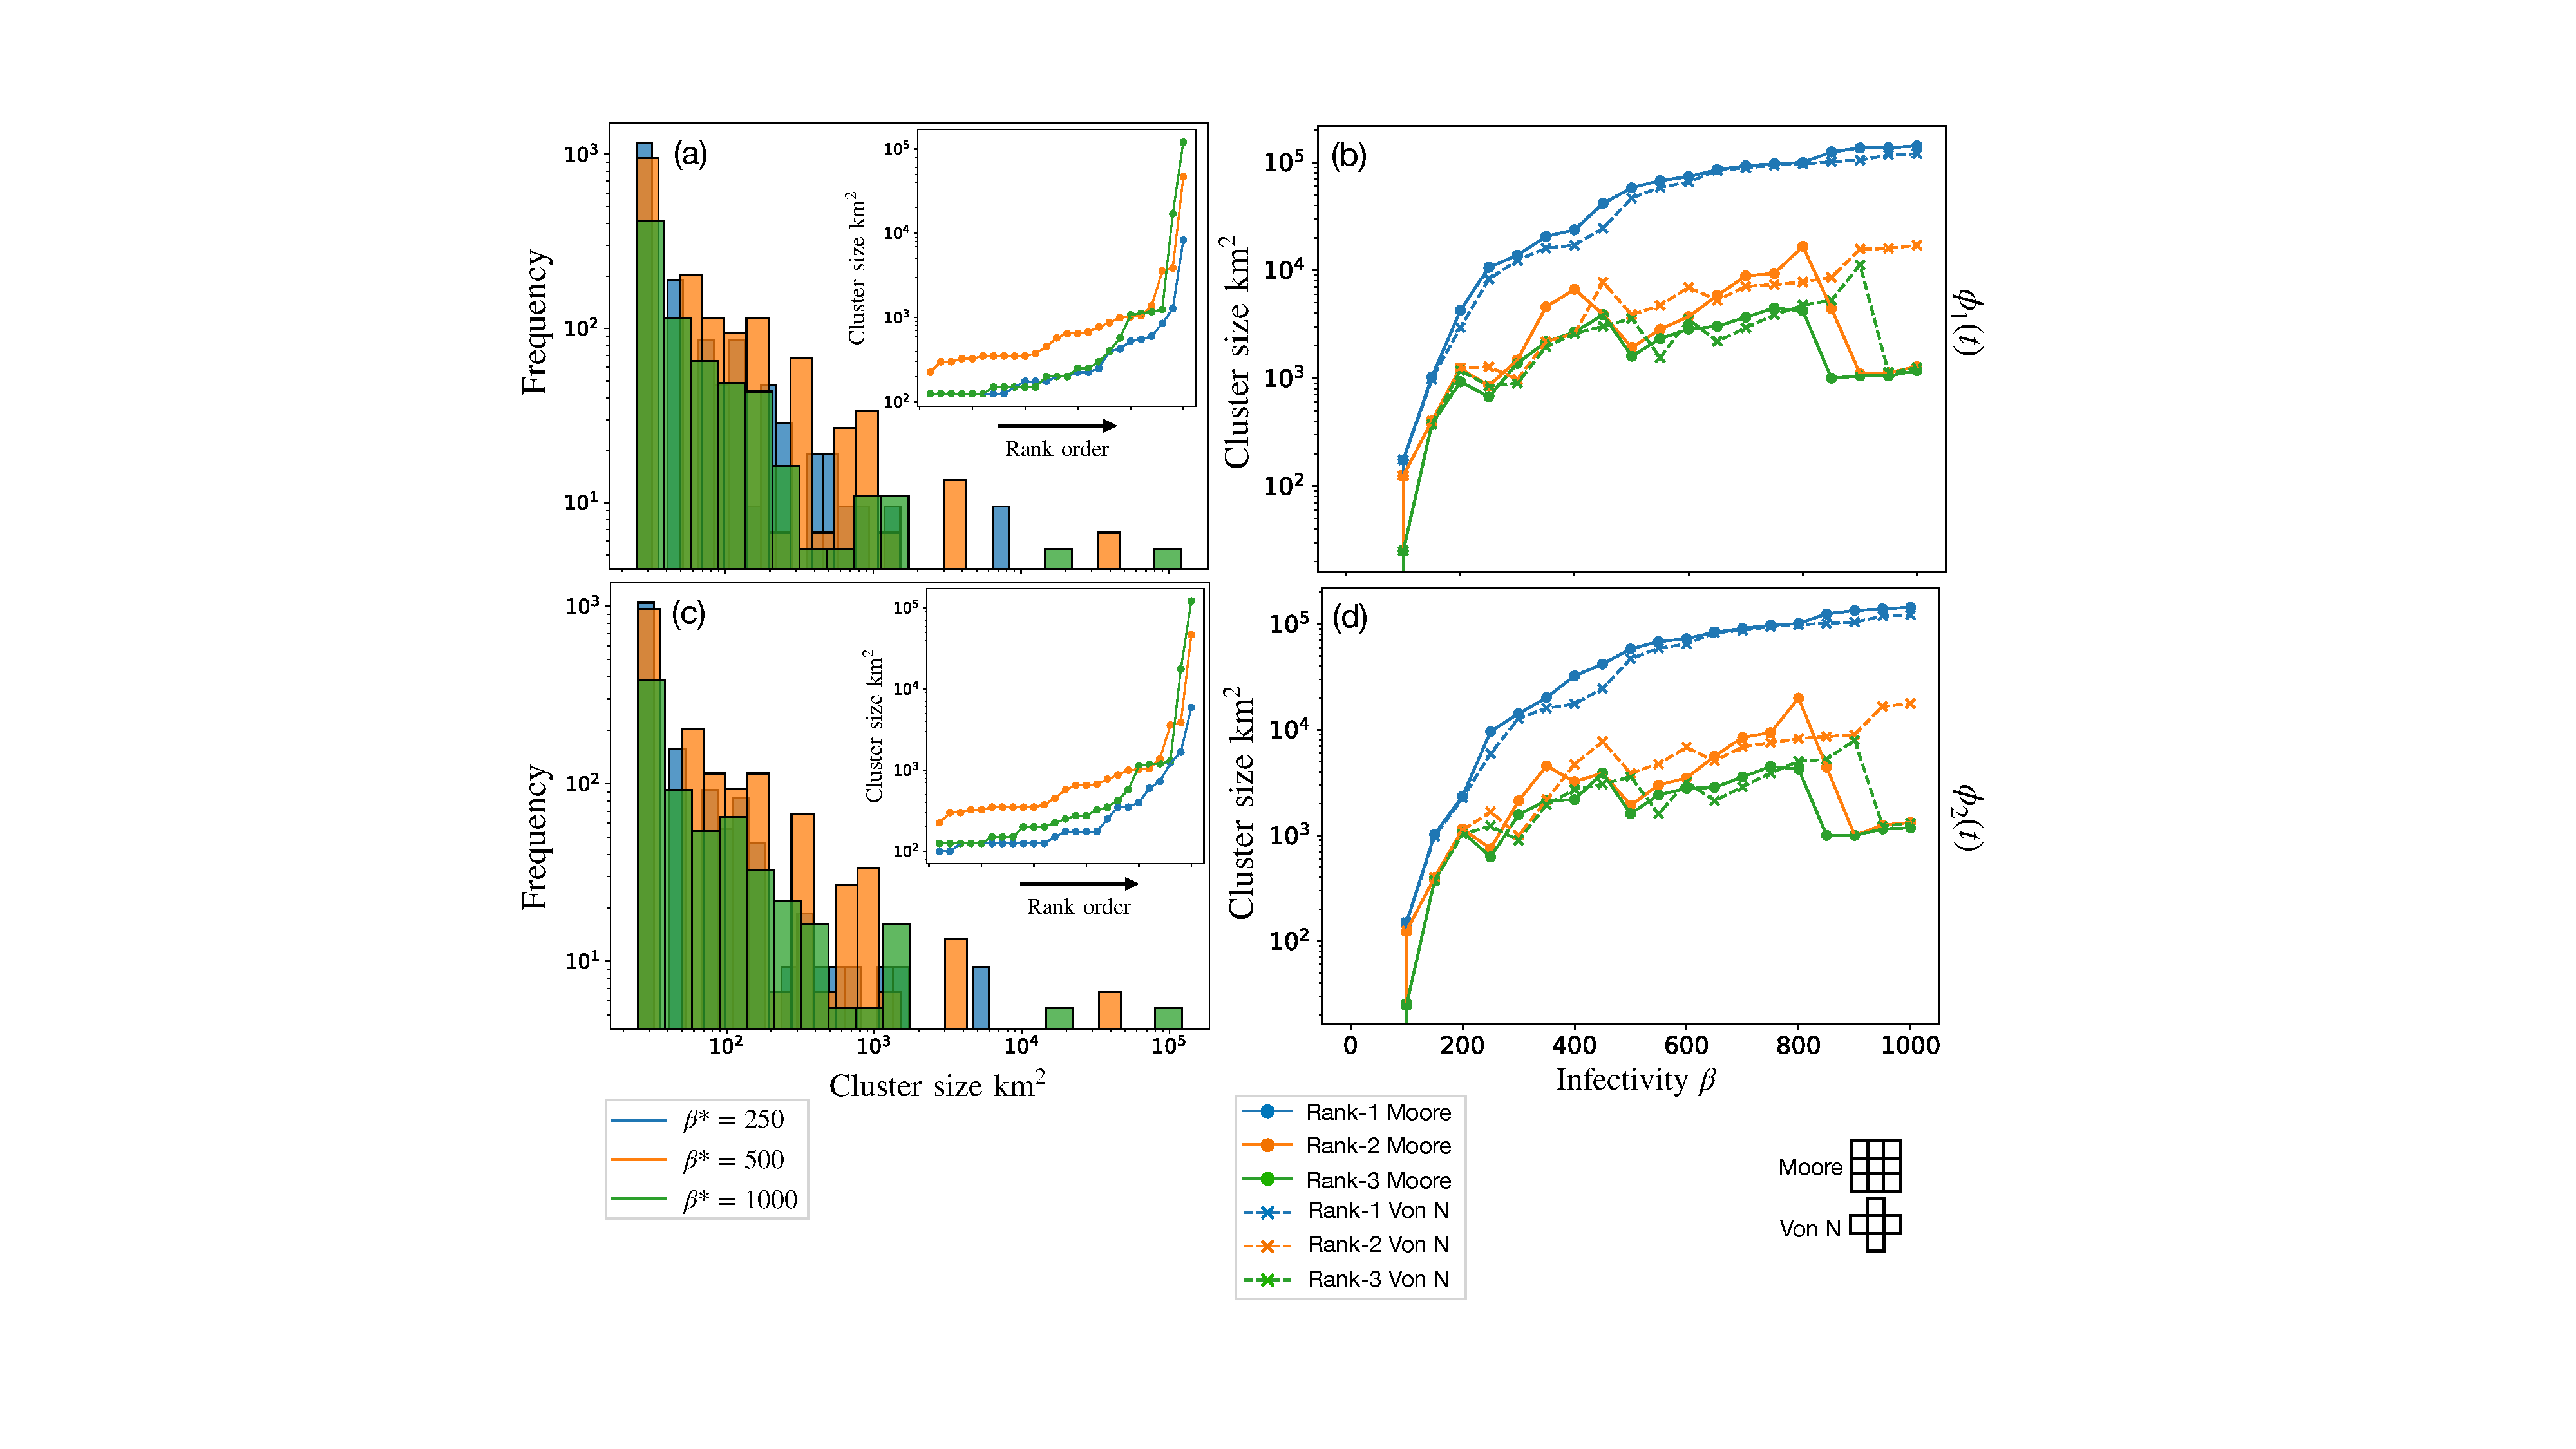
\includegraphics[scale=0.45]{chapter6/figures/fig6-pl-cluster-distribution.pdf}
    \caption{Susceptible $R_0$-clustering for the inverse power law model (a) For model $\phi_1$-pl, the cluster-size frequency distribution is shown for three infectivity values utilising the Moore neighbourhood. The inset shows a rank-ordered graph of the top $25$ most significant clusters by area $\mathrm{km^2}$. (b) The top three ranked clusters, by size, for model $\phi_1$-pl is shown over the infectivity parameter-space for both Moore and Von-Neumann neighbourhoods. (c) The frequency distribution of cluster size is shown for the peaked sporulation model $\phi_2$-pl for three infectivity parameters (d) Cluster-size behaviour for model $\phi_2$-pl shown over infectivity parameter-space for Moore and Von-Neumann neighbourhoods.}
    \label{fig:inverse-power-law-clustering}
\end{figure}

In the $SEIR$ model, a value of $\beta$ has not been determined by statistical fitting.
Therefore, we are compelled to study behaviour over the entire space of $\beta$.
Figures \ref{fig:inverse-power-law-clustering}(b) and (d) describe how $R_0$-clusters scale over different values of infectivity and structuring elements for models $\phi_1$-pl and $\phi_2$-pl respectively.
As infectivity is increased to a maximum of $\beta^*=1000$, the largest $R_0$-cluster (shown in blue) rises most rapidly over a narrow range of infectivity values in the interval $\beta^*\in [100, 400]$.
Patches are more likely to become susceptible as $\beta^*$ increases; this causes rank-1 $R_0$-clusters to amalgamate surrounding neighbouring clusters as channels open up.
Thus, fluctuations arise in the second and third largest clusters as they form an ever-larger dominating cluster.
Below $\beta^*=100$, no cluster-growth is displayed as epidemic parameters are too low. 
 
Up to this point, we have considered one structuring element, namely the Moore neighbourhood.
The type of structuring element we choose to gauge regional-susceptibility in the $R_0$-map bears no influence on how an epidemic might progress in reality.
Therefore, it is desirable for clustering in the model to remain invariant over the structuring element we choose.
In general, visible, albeit small, differences can be seen due to artefacts of the structuring elements.

Moore neighbourhoods can be seen to produce slightly larger rank-1 $R_0$-clusters, which in turn reduced the size of second and third-ranked clusters.
The disparity caused between structuring elements can be understood by noting the two additional corner/diagonal pieces in the Moore neighbourhood.
Although structuring elements account for a comparatively small deviation between cluster sizes, the rank-1 clusters compared similarly for some values for $\beta^*$.
Observing minor artefacts due to structuring elements hint toward limitations in the definition of connectivity, as defined within the landscape-level component of the model.

\subsection{Gaussian $R_0$-map clustering: varying map resolution}
\label{sec:gaussian-r0-clustering}

The essential dynamic of $R_0$ clustering holds when spatially scaling the Gaussian-based models $\phi_1$-ga and $\phi_2$-ga.
Notwithstanding some negligible cluster size differences, as demonstrated above in Figure \ref{fig:R0-map-generation}.
However, as explored in section \ref{sec:r0-vs-L}, $R_0$-values in the more localised Gaussian dispersal models can be discerned inside a domain size of $\mathrm{1km \times 1km}$.
Given that $R_0$ can be captured inside a smaller domain, we may consider resolving $R_0$-maps to a finer landscape-level resolution in comparison to the inverse power law-based dispersal models.
Resolving $R_0$-maps to the highest resolution possible is desirable to apprehend the nature of epidemic severity and spatial heterogeneity.
Otherwise, relevant epidemic information is lost when coarse-graining the host distribution. 

Figure \ref{fig:gaussian-clustering} shows how CCA changes clustering in the $R_0$-map for different landscape-level resolutions.
Figures \ref{fig:gaussian-clustering}(a-c) show the frequency distributions of cluster size for $\beta^*=500$ and three different patch sizes, of lengths $\mathrm{5km,\ 3km,\ 1km}$ respectively.
As discussed in section \ref{sec:inverse-power-law-r0-clustering}, the same general trend remains, i.e. a small number of large clusters alongside more numerous small clusters.
Although, decreasing the patch size produces a more fragmented domain, indicated by the greater variety of cluster sizes.
The largest ranked cluster toward the far-right of each distribution also shrinks for successively smaller patch sizes.
However, decreasing the patch size brings frequency distributions between structuring elements into closer alignment, seen by a closer agreement of blue and orange distributions in Figure \ref{fig:gaussian-clustering}(c).

As before, cluster size for the largest ranked cluster exhibits the most significant growth over the first few values of infectivity, $\beta^* \in [100, 400]$.
However, performing CCA at different landscape-level resolutions produces a change in the size of $R_0$-clusters.
At the most extreme point of $\beta^*=500$, more significant deviations can be seen between the size of rank-1 susceptible $R_0$-clusters, illustrated by the vertical arrow in Figure \ref{fig:gaussian-clustering}.
Figures \ref{fig:gaussian-clustering}(e-g) depict visual differences of CCA at domain resolution $\mathrm{5km \times 5km, 3km\times 3km}$ and $\mathrm{1km\times 1km}$.

Similar landscape-level features in the $R_0$-maps are witnessed for each domain resolution considered.
Nevertheless, disparities exist in cluster size at different landscape-level resolutions.
As the $R_0$-map is resolved to a small spatial-scales, connectivity within an $R_0$-cluster can depend more critically on a small number of above-threshold patches, identified by the red circles in the inset in Figure \ref{fig:gaussian-clustering}(c).

In the coarse-grained domain of Figure \ref{fig:gaussian-clustering}(e), the critically-connecting patches circled in Figure \ref{fig:gaussian-clustering}(g) 
are smoothed in the process of averaging the small number of surroundings patches. 
Similarly, some above-threshold patches can be smoothed to below-threshold patches, thus increasing the cluster size, shown in Figure \ref{fig:gaussian-clustering}(b) circled in red.
Ultimately, differences in cluster size are caused by the simplistic notion of connectivity within CCA that fails to scale with the domain resolution.
Witnessing a difference in CCA-identified clusters is not desirable and outlines an inherent limitation of the framework.
Even though clusters appear different, these observations emphasise that connectivity over a region can depend on a small number of patches, 
which sets the scene for chapter \ref{ch7:landscape-level-control}.

\begin{landscape}
\begin{figure}
    \centering
    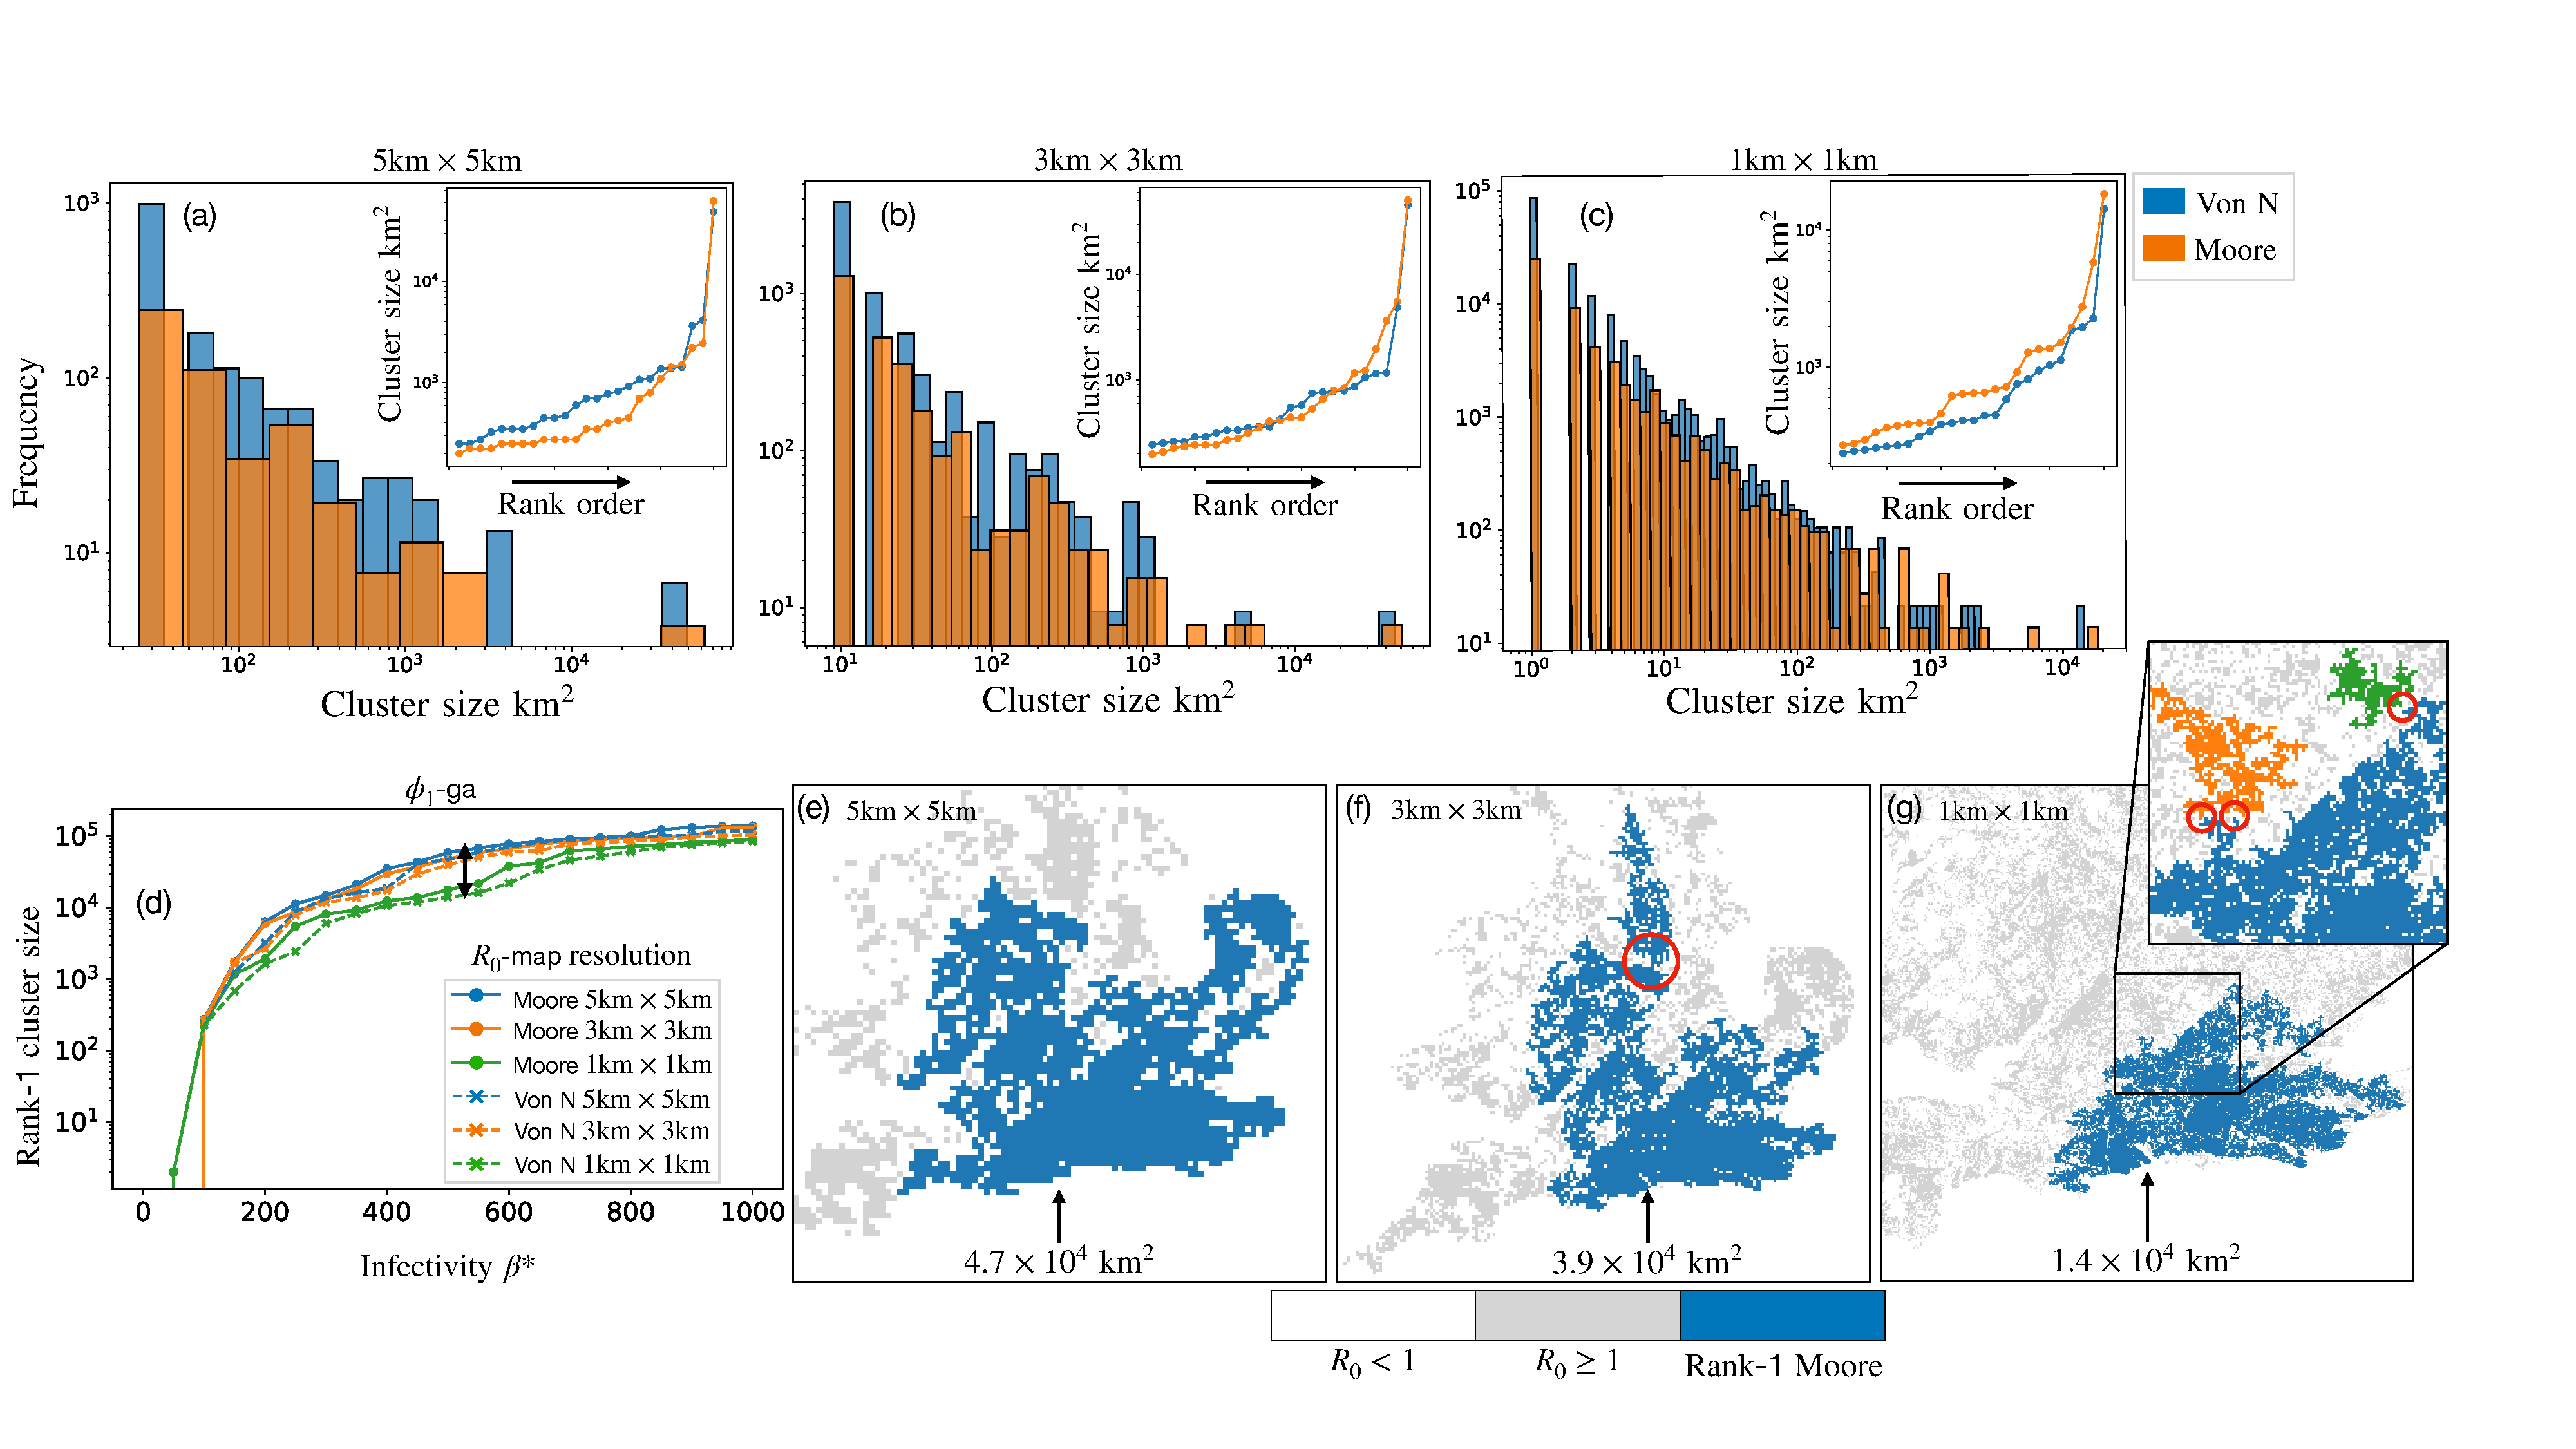
\includegraphics[scale=0.395]{chapter6/figures/fig6-ga-cluster-distribution.pdf} 
    \caption{Multi-scale CCA performed over different landscape-level resolutions, namely from $\mathrm{1km \times 1km}$ to $\mathrm{5km \times 5km}$ patch-sizes. (a-c) Cluster-size distributions are shown for three landscape-level domain resolutions and both Moore and Von-Neumann structuring elements. As domain resolution is increased to $\mathrm{1km \times 1km}$, clusters can be resolved to a finer scale and yield a set of clusters over more length-scales (d) Cluster sizes over infectivity $\beta^*$ and structuring elements, comparing behaviour at two pixel-sizes. At the most extreme point, large disparities in cluster sizes become apparent, indicated by the vertical arrow at $\beta^*=500$. (e-g) Spatial interpretations of cluster-size deviations at different domain resolutions according to the Moore neighbourhood at $\beta^*=500$.}
    \label{fig:gaussian-clustering}
\end{figure}
\end{landscape}

\section{Chapter summary}

The work presented in this chapter describes how to project a spatially explicit, small-scale compartmentalised model onto a host distribution.
The method to `spatially scale' a small-scale epidemic model is computationally inexpensive, flexible and generalisable.
Results are focused on helping policymakers implement informed decisions about \textit{where} to control the spread of disease, based on spatial arguments.
In the face of low budgets, limited resources and short decision windows, an efficient method to prioritise targeted control could aid both policymakers and forest managers\textemdash as noted by \cite{13-challenges, time-varying-infectivity}.

Given the sessile nature of trees, the spatial distribution of hosts remains of paramount importance for epidemic modelling.
As such, a modelled distribution of ash covering Great Britain was used to parameterise host densities.
This choice was motivated by the non-existence of freely available, high-quality ash abundance data that spans Great Britain.
Consequently, combining our small-scale $SEIR$ model with data given by \cite{hill.data} demonstrates a novel use of modelled abundance data\textemdash
as remarked when summarising the toy SLM model of chapter \ref{chapter:SLM-applications}.

Due to the complexity of ADB, some important assumptions had to be employed in the $SEIR$ model.
In particular, leaf-shed was assumed to fall close to ash hosts; 
this permitted fungal ascospore dispersal to originate from the same location as infected ash.
Still, this assumption is supported by the dispersal parameterisation given by \cite{grosdidier2018tracking} that measured dispersal directly between a source of infected trees and spore-traps, thereby omitting the dynamics of intermediary leaf-shed dispersal.
One possible improvement to the $SEIR$ model might include host demography, as host-pathogen coexistence is not supported.

Performing CCA proved a beneficial yet problematic exercise.
Multi-scale CCA demonstrated how failing to include relevant epidemiological information, in the form of coarse-grained host data, can lead to significant disparities in cluster size\textemdash sentiments echoed in the third challenge posed by \cite{13-challenges}.
Furthermore, resolving Gaussian $R_0$-maps at different landscape resolutions emphasises an implicit assumption when defining connectivity based solely on nearest-neighbour interactions between patches. 
That is, Moore and Von Neumann structuring elements do not scale with the dispersal kernel under a change of map resolution:

\textit{Suppose secondary infections can be induced up to a maximum distance of $D_{max} = 2\mathrm{km}$.
Resolving the map to $\mathrm{2km \times 2km}$ (or lower) is permissible because patches interact locally i.e. infections between non-nearest neighbour patches are unlikely (neglecting atmospheric of human-mediated LDD).
In contrast, suppose the map is now resolved to $\mathrm{1km \times 1km}$.
In this scenario, patches have the possibility of interacting non-locally because $D_{max}$ exceeds intermediary patches;
nearest-neighbour structuring elements therefore fail to describe connectivity accurately.}
Given all the above, an improved understanding of the connectivity between patches is required to progress the framework.

In a nutshell, multi-scale CCA questions the very notion of constructing $R_0$-maps for systems described by fat-tailed dispersal kernels.
The invasiveness of a pathogen described by a fat-tailed dispersal kernel cannot be defined by $R_0$ reliably inside a small domain.
Therefore, epidemic maps depicting inverse power law $R_0$-values require a larger patch size that motivates a coarse-grained host distribution, lowering map resolution.
Omitting finer-scale epidemic information can lead to disparate results, witnessed by varying the Gaussian-based $R_0$-map patch-size.
Thus, mapping $R_0$ values for inverse power law dispersal is called into question.

Despite the limitations of CCA, clusters grew up to four orders of magnitude over the initial interval of infectivity, $\beta^*\in [100, 400]$.
Rapid cluster growth between $\beta^*\in [100, 400]$ occurred for all $SEIR$ model-variants and domain resolutions considered.
Landscape-level spread within our framework, therefore, demonstrates a threshold-like behaviour, below witch ($\beta^* \lessapprox 100$), no models would be able to invade Great Britain.
The next valuable step would be to fit a value of $\beta$ to data on ADB spread\footnote{Given the high availability of ADB mortality data in different European countries, fitting the $SEIR$ model to mortality curves would be most accessible.}, 
and construct the resulting $R_0$-map.

% \section{Chapter summary}

% Where we consider spatial structure and others have not
% - In this chapter, we focused on disrupting local-level dispersal by implementing control at landscape-level.
% -  In this chapter we undertook the ambitious task of scaling up a small-scale model, to large spatial distances covering GB, and developed a new approach to controlling the spread of disease.
% - introduce the regime of pathogen spread we are interested in, we are not modelling continental long-range spread via upper atmosphere, nor are we interested in long-range human trade networks. We are interested in dispersal at the local level whereby passive means of wind, soil and or insects/animals. 

% link to 13 challenges: -- it is your friend...
% 1 - host data is hard to integrate into models \cite(13 challenges), we demonstrate how how this can be achieved
% 2. primed a model of multi scale, although we have not included LDD spore transport, the framework serves to include this via a more complete treatment of the structuring element
% 3. capturing time-varying infectivity is hard \cite{13 challenges},
% 4. constructing a spatial model of disease severity could help to deploy resources to known locations e.g. monitoring
%5. web api to help policy makers

% The work conducted in this chapter are focused toward help policy makers implement informed decisions, about \textit{where} to control the spread of disease, based on spatial arguments.
% The framework we implemented was constructed using a simplified model of ADB, although the method is flexible and can be generalised for other compartmentalised models, provided sufficient host data and fitted epidemiological parameters. 
% In the face of low Identifying which locations are likely to support the highest epidemic severity is key for targeted control when budgets are low\textemdash as noted by \cite{time-varying-infectivity}. Our approach of spatially scaling small-scale epidemiological principles was conducted through computational, opposed to analytical, means. 

% % The scaling up of our model
% The scaling up of our model resembles a metapopulation model, now commonplace when modelling plant-based epidemics, but crucially our large-scale model is not dynamic. A dynamic large-scale model is indeed useful for the prediction of time-scales and the movement of disease-fronts movement; however, we suggest they might be at best less useful for optimised large-scale control, and at worse, nicely complemented by the approach we develop.

% If early data through a particular region, with known data, was collected, it would be a relatively short step to fit the dispersal model and scale up the model over large distances given the seemingly simple relation to host density $\rho$.
% % At the small scale we have a uniform population. However for larger scales we have considerable spatial heterogeneity.
% % spatial-scale and control, over a multi-seasonal pathosystem, have been investigated for sugar beet in the UK, see \cite{doi:10.1146/annurev.phyto.45.062806.094357} for a review.


% % On the SEIR model

% The cyclic nature of the $SEIR$-type model constructed in this article can also find resemblance in the, well established body of literature, of crop-based epidemics. It is common-place for a field of crops to become infested, then at the end of the growing season be totally eradicated by virtue of harvesting 
% % there is a surprising lack of, simplified, ash dieback models in the literature...\ciations... <-- double, triple and quadruple check!
% % without host demography 
% % landscape level control strategy
% % Therefore, not modelling the asexual component of ADB represents an important assumption in the model.
% % , both spatial and genetic variations are known to influence the epidemic progression of ADB \cite{stocks2017first, mckinney2014ash}. 
% % Observations of ADB invasions suggest a strong on the surrounding landscape features \cite{https://doi.org/10.1111/1365-2745.13383}.
% % Here, the function $\phi_2(t)$ is a special case of the Gamma(k) presented in \cite{time-varying-infectivity}.

% % Adopting a compartmentalised $SEIR$-like structure to model the spread of ADB at local spatial-scales is both novel and ambitious
% % \footnote{Models of plant-based fungal pathogens with comparable life-cycles have typically opted for different approaches e.g. the ascomycete `apple scab' \cite{rossi2007scab}}.

% % Fitting the seasonal $SEIR$ model of ADB to ash mortality data would therefore be most tenable. In practice, fitting could be explored by varying $\beta$ until the mortality curve resembles experimental data

% % multi-scale approaches have been outlined \cite{hart2020theoretical}
% % multi-seasonal frameworks comprise a common theme in the spread of crop-based epidemics see  x, y, and typically involve soil-borne nematodes-based outbreaks \cite{tankam2020modelling} <- see references inside.

% % \cite{time-varying-infectivity} has 
% % we contend the SnIEmR model, considered over one sporulation peak, is a simplistic implementation of the SEIR-based model needed to compute an invasion threshold that represent the infection dynamics ash dieback. 
% % The SEIR-based model is made more flexible, and can be readily extended or adapted to incorporate more biological realism, by virtue of splitting the E and I into multiple compartments\textemdash this is frequently done in human and animal-based models \citations..

% % - time varying infectivity parameter for ADB \beta could be subject to increase in response to the warmer conditions presented by climate change \cite{magarey2005simple}
% % - Interestingly, ash dieback could be adversely effected be climate change \cite{goberville2016climate}


% %- Although the main result of our work was conduced over one sporulation peak, or life-cycle of ash dieback, splitting the model into various compartments was a useful and necessary step towards developing accurate large-tree species. reference  \cite{https://doi.org/10.1111/ppa.12894} alludes to multiple exposed periods being useful

% %- A quantity of interest that appears frequently in the literature is the initial growth rate $r$, that is the density-independent growth at the start of any epidemic.
% % See \cite{ferrandino2012time} for a review on the time-scales and sporulation of plant-based diseases.

% % Fitting data to the early phases of an epidemic has been shown to give large differences in the final-size epidemic, or severity \cite{time-varying-infectivity}. However, we are only interested in a pathogens ability to invade and this can be closely approximated by measuring R0 over the fist observation (\see appendix)
% % fitting....- Although, various data regarding ash mortality after years of infection have been published in various countries, as reviewed in chapter \ref{ch2:ash-dieback}.
% % The variability between the particular life-cycle history followed by hosts is thought to be an important factor to consider\cite{ferrandino2012time}, and we intentionally neglected this for the purpose of simplicity...

% % subdividing compartments in this manner could also provide an easier implementation to hosts which become more infectious, through a greater production of spores, as the infectious cycle continues not to mention particular periods of environmental unsuitability.
% %

% % Accurately modelling time-varying infectivity is difficult \cite{13-challenges}, and as such, we opted for parsimony.

% % Main assumptions in the method: 
% % 1) Assumptions about dispersal
% Dispersal over small spatial-scale is thought to predominately occur passively through wind, however other means of dispersal exist such as soil and or insects. There are many pathways a pathogen can use to spread through a landscape, including long-range dispersal, mediated through either human-trade networks %
% \cite{hulme2009trade, banks2015role, chapman2017global} or dispersal in the upper atmosphere \cite{westbrook1999atmospheric, isard2005principles}.  

% % \textcolor{red}{The last insightful observation from Figure \ref{fig:max_dist_vs_R0} relates to the averaging spreading velocity of ADB...}
% % We assumed some regions can sustain an epidemic and some cannot, we assume that $R_0>1$ is the threshold separating these regimes.

% % 2) Assumptions about R0
% To our knowledge, $R_0$ has not been estimated for Ash dieback, or indeed for any large deciduous tree species, unlike for some crop-based pathogens \cite{segarra2001epidemic}. The lack of $R_0$-estimates made it hard to scrutinize which $\beta$-valued $R_0$-map would be likely to reflect reality. This gap in the body of literature is hardly surprising given the complexity of measuring time-varying infectivity rates \cite{13-challenges}. Thus, as it stands, our results hint-towards the utility of landscape-level control but come short of definitive proof.

% % Looking at \cite{R0-perc-ref}, it makes me think our notion of $R_0$ is pretty simplistic. We only measure the local-level $R_0$. We do not consider $R_0$ from patch to patch. What scale we measure $R_0$ has a huge impact on what the result is. Could we rank land-patches not only on there local $R_0$ level, but also on the impact they have on there immediate neighbours ? This would, in theory be an improvement to the clustering algorithm.

% % A map of $R_0$ values is useful to policy makers and plant modelers alike.

% % Improvements to the model:
% % 1) The algorithm
% % The algorithm to target not only the critically connecting patches, but also find fragmenting lines which minimise risk at the landscape-level ? Incorporating the local impact a particular patch may have on its neighbours.
% % 2) Multi-year R0 analysis
% % However, we .... xyz cover all basis of using a one-season approximation. <- this leads to a risk-based argument in which we could capture a 2nd-order R0 which does, xyz. We mainly interested in a pathogens ability to invade. 

% % Analysis was aired towards simplicity, a more expansive study with e.g. more sophisticated sporulation functions could be the subject of future work.

% % The most important message of our work was...
% % The spatial and temporal scale of the control-strategy should match intrinsic spatial and temporal scale of the invasion. <- Hence R0 measured over one season. 

% \textbf{Assumptions}
% \begin{itemize}
%     \item Infectious, dead leaf litter was assumed to fall close to infected ash, and ash were taken as the site of fungal dispersal. In reality dead leaves could themselves disperse. 
%     However, the dispersal parameterisation from \cite{grosdidier2018tracking}
%     Omitting leaf dispersal simplified the model and given informed parameterisation by from \cite{grosdidier2018tracking} bared no influence the scale of dispersal
%     \item leaf dispersal has been studied by \cite{https://doi.org/10.1890/0012-9658(2006)87[2306:MLDIMH]2.0.CO;2, staelens2003model}
%     \item no host demography link to $R_0$
%     \item The transition probability $\beta$ is constant throughout the life-time of infected ash. 
% \end{itemize}

% % our modelling approach and results are in their infancy,  

% % Last remarks and future modelling work:
% To our knowledge, there is a surprising lack of spatio-temporal ADB models exist in the literature, probably because of the significant challenges involved in containment. Although our findings are far from complete, it suggests the spread of ash dieback, between spatial locations, could be reduced by preferentially targeting sites to minimise epidemiological connectivity. Not surprisingly, more work will need to be done to ascertain the degree to which this strategy could impede the spread. 



